%%%%%%%%%%%%%%%%%%%%%%%%%%%%%%%%%%%%%%%%%%%%%%%%%%%%%%%%%%%%%%%%%%%
%                                                                 %
%   MINUIT User Guide -- LaTeX Source                             %
%                                                                 %
%   Part 2: Tutorial Section                                      %
%                                                                 %
%   The following external EPS files are referenced:              %
%      mi1.eps, mi23.eps, mi4.eps through mi14.eps                %
%                                                                 %
%   Editor: Michel Goossens / CN-AS                               %
%   Last Mod.:  2 jun. 1992 10:00 mg                              %
%                                                                 %
%%%%%%%%%%%%%%%%%%%%%%%%%%%%%%%%%%%%%%%%%%%%%%%%%%%%%%%%%%%%%%%%%%%

%               FUNCTION MINIMIZATION
%        Reprinted from the Proceedings of the
%  1972 CERN Computing and Data Processing School,
% Pertisau, Austria, 10-24 September, 1972 (CERN 72-21)
\def\UTG{\lower.8ex\hbox{$\sim$}\kern-.8em\raise.25ex\hbox{$G$}\;}
\def\UTI{\lower.8ex\hbox{$\sim$}\kern-.8em\raise.25ex\hbox{$I$}\;}
\def\UTV{\lower.8ex\hbox{$\sim$}\kern-.7em\raise.25ex\hbox{$V$}\;}
\def\UTA{\lower.8ex\hbox{$\sim$}\kern-.8em\raise.25ex\hbox{$A$}\;}
\def\UTI{\lower.8ex\hbox{$\sim$}\kern-.6em\raise.25ex\hbox{$I$}\;}
\def\UTd{\lower.8ex\hbox{$\sim$}\kern-.8em\raise.25ex\hbox{$d$}\;}
\def\UTf{\lower.8ex\hbox{$\sim$}\kern-.7em\raise.40ex\hbox{$f$}\;}
\def\UTT{\lower.8ex\hbox{$\sim$}\kern-.8em\raise.25ex\hbox{$T$}\;}
\def\UTD{\lower.8ex\hbox{$\sim$}\kern-.8em\raise.25ex\hbox{$D$}\;}
\chapter{Introduction}
\section{The motivation}
 
A large class of problems in many different fields of research can
be reduced to the problem of finding the smallest value taken on by a
function of one or more variable parameters.  Examples come from fields
as far apart as industrial processing (minimization of production costs
and general relativity (determination of geodesics by minimizing the
path length between two points in curved space-time).  But the classic
example which occurs so often in scientific research is the estimation of
unknown parameters in a theory by minimizing the difference (chi-square)
between theory and experimental data.  In all these examples, the function
to be minimized is of course determined by considerations proper to
the particular field being investigated, which will  not concern us in these lectures.
Our aim is to study the mathematical problem of minimization.
 
\section{Minimization, maximization, and optimization}
 
Although traditionally one speaks of function {\em minimization}, some
authors refer to {\em maximization}.  Of course the two are entirely equivalent
since one can be converted to the other by changing the sign of the function.
Thus the problems of minimizing chi-square, maximizing likelihood,
minimizing cost, or maximizing efficiency can all be considered as
minimization (or maximization).  To avoid committing oneself, it is now 
fashionable to speak of {\em optimization}, to cover both cases.  This
unfortunately causes confusion with optimization in control theory where
the principal techniques are analytical (calculus of variations) and
hence bear little relationship to the numerical methods used in function
minimization as treated here.
 
To add to the confusion there is the term `programming', which is
also used to mean minimization (usually specified as {\em linear programming,
non-linear programming,} or {\em mathematical programming}), a historical usage
dating from the time when programmers in the modern sense did not exist,
and computer users were not programming but coding.
 
Other terms used for minimization are {\em extremization} and
{\em hill-climbing}.  Since these can also be used to mean other things, the
general conclusion is that in this field you can not tell a book from
its title.  While waiting for general agreement as to what the subject
should be called, we will stick to function minimization.
 
\section{Definition of the problem}
 
      Given a function $F(x)$, the general problem is to find the value of
the variable or variables $x$ for which the function $F(x)$ takes on its
smallest value.  [As pointed out above, this is entirely equivalent to
finding the $x$ for which the function $-F(x)$ takes on its largest value,
but for consistency we will always consider only minimization.]  The
rules of the game are the following:
 
  i) The function $F(x)$ is assumed not to be known analytically, but is
     specified by giving its value at any point $x$.
 
 ii) The allowed values of the variable or variables $x$ may be restricted
     to a certain range, 
     in which case one speaks of constrained
     minimization.  In these lectures we limit ourselves to the
     unconstrained problem.
 
iii) In some cases additional information about the function $F$ may be
     available, such as the numerical values of the
      derivatives $\partial F/\partial x$ at any point $x$.
     Such knowledge cannot in general be assumed, but
     should be used when possible.
 
 iv) The function $F(x)$ is repeatedly evaluated at different points $x$
     until its minimum value is attained.\\ \noindent
 The method which finds the minimum (within a given tolerance) after the
fewest function evaluations is the best.  Occasionally other considerations
may be important, such as the amount of storage required by the
method  or the amount of computation required to implement the method,
but normally the dominating factor will be the time spent in evaluating
the function.
 
 
\section{Definition of a minimum}
 
     The theorems of elementary calculus tell us that the function
$F(x)$ must take on its smallest value at a point where either:
 
  i) all derivatives $\partial F/\partial x = 0$ (a {\em stationary point)}, or\\ \indent
 ii) some derivative $\partial F/\partial x$ does not exist (a {\em cusp}), or\\ \indent
iii) the point $x$ is on the boundary of the allowed region (an {\em edge point}).
 
     Although we will sometimes find it useful to consider points
satisfying the above properties, this approach of considering essentially
the analytic properties of the function is clearly not well adapted to
the rules of the game as outlined above.  Indeed, when one considers that
there may be any number of stationary points, cusps, and edge points,
all of which may be arbitrarily hard to find by simply sampling the
function value, the whole problem begins to appear hopeless unless some
simplifying assumptions are made.
 
     The usual simplification consists in abandoning the attempt to find
the {\em global minimum} and being satisfied with a {\em local minimum}.  A local
minimum may be defined as a point $x_0$, where for all points $x$ in some
neighbourhood around $x_0$ we have $F(x) > F(x_0)$.
 
     Now the situation looks much brighter since the very definition of
a local minimum suggests a general strategy for finding one:  we vary $x$
by small steps in a direction which causes $F$ to decrease, and continue
until $F$ increases in all allowed directions from some point $x_0$.
This
does not yet tell us how to vary $x$, but at least it suggests that a solution
can be found.
 
In the lectures we will consider only unconstrained local minimization, unless otherwise stated.
The problem of global minimization will be treated in Section~6.
 
 
\section{The shape of the function -- Taylor's series}
 
     With a view to making an intelligent minimizing method, it is of
interest to consider what we might reasonably expect about the behaviour
of $F$.
If $F$ represents a physically meaningful function, we would certainly
expect all the derivatives of $F$ to exist everywhere in the region of
interest.  Under these conditions we can write down the {\em Taylor's series}
expansion for $F$ about some point $x_1$, assuming for the moment that $x$
represents just one variable:
 
$$\left .F(x)~=~F(x_1)~+~{\partial F\over \partial x}\right
|_{x_{1}}~(x~-~x_{1})~+~{1\over 2}~\left .{\partial^{2}F\over \partial x^2}\right
|_{x_{1}}~(x~-~x_{1})^{2}~+~\ldots~.$$
 Although we do not know anything {\em a priori} about the domain of convergence
of this series, we do know that as the distance $(x - x_1)$ becomes smaller,
the higher order terms become less important, so that we would expect
that predictions based on the low-order terms should not be very wrong,
at least for small steps.  Before considering these terms in more detail
let us generalize the variable $x$ to a vector of n variables $x$.  Then we
have
 
$$F({\underline{x}})~=~F({\underline{x}}_1)~+~{\underline{g}}^T({\underline{x}}
~-~{\underline{x}}_1)~+~{1\over 2}~({\underline{x}}~-~{\underline{x}}_1)^T~\UTV({\underline{x}}
 - {\underline{x}}_1)
+~\ldots~,$$
where the matrix $\UTV$ is defined by $G_{ij} = \partial^2 F/\partial x_i
\partial x_{j}$ and
          the gradient vector ${\underline{g}}$ is $g_i = \partial F/\partial x_i$, all
derivatives
          being evaluated at ${\underline{x}}_1$.  The $T$ denotes transposition
          which turns a column vector into a row vector.  Note
          the difference between $x_i$ (the $i^{th}$ variable) and ${\underline{x}}_i$
          (the position vector at the point $i$).
 
Now the first term of the above series is constant, so it will not tell
us much about where to look for a minimum.  The second term is
proportional to the gradient  ${\underline{g}}$
and tells us in which direction the function is
decreasing the fastest, but since it is linear in ${\underline{g}}$, it does not predict
a minimum and therefore does not tell us what step size to take.
Moreover, as we approach the minimum ${\underline{g}}~\to~0$ (if it exists)
so we will have to
go further and consider the next term.  The third, or quadratic term
describes a parabolic behaviour and is therefore the lowest term to
predict a minimum.  Unlike ${\underline{g}}$ we can expect $\UTV$ to be roughly constant over
small regions, since it would be exactly constant if higher-order terms
were zero.
 
     We mention, in passing, one class of problems in which the above
analysis would not hold at all.  This is in the field known as linear
programming, which limits itself to minimizing functions which are linear
in the parameters, subject to constraints which are also linear.  A
linear function can not have a minimum in the sense described above (a
stationary point) but must take on its minimum at a constraint boundary
(edge point).  For such problems the description of the constraints therefore
takes on greater importance than the analysis of the function
itself, and will not be considered in these lectures.
 
 
\section{Non-existence of optimum in general}
 
     Although we will be studying and comparing
different minimization algorithms (recipes), the reader should be warned
at the outset that in the strict sense of the rules of the game as stated
in Section 1.3 above, we will not be able to show any algorithm to be
superior to any other for all functions.  In principle at least, no
matter how bad one algorithm is, or how good another, we can always find
a function which will be minimized faster by the bad method than by the
good one.  We should keep such essentially theoretical considerations in
mind, but should not be overly discouraged by them.  In particular,
certain objective criteria will emerge for comparing methods even though
the principal criterion---minimization speed---depends on the function.
In the past there has in my opinion been an overemphasis on such objective
criteria in an attempt to find the ideal universal minimization
algorithm.  More recently, the tendency is to adapt the algorithm to
the function, even to the point of introducing a super-algorithm which
would
choose a sub-algorithm appropriate to the function at hand. Such questions
of global strategy will be considered later.
 
     The reader should also be warned that in presenting particular
algorithms I will often omit details which are unimportant to an
understanding of the algorithm although they may be crucial in actually
making it work.  The original references should therefore be consulted
before programming such algorithms.
 
 
\section{The role of the computer}
 
     While our subject is essentially a mathematical one, it has been so
profoundly influenced by the existence of high-speed electronic computers
that it would certainly be unfair  not to mention them here.  Indeed,
real progress in the solving of large-scale practical problems has come
only since the 1960's, although much of the basic theory dates
back to Newton's time or even earlier.  This is, of course, because of
the renewed interest in numerical minimization techniques for use on
computers.  As it is no longer even thinkable to use these techniques
for hand calculations, it is best to place ourselves immediately in the
computer context and to conceive of our function $F(x)$ rather as a
subroutine which returns a value of $F$
(and perhaps some other information
such as numerical values of derivatives) for given input values of the
arguments $x$.
 
     One unpleasant consequence of the computer-oriented approach is that
we will often have to worry about rounding-off errors in the
function value due to the finite word length of digital
computers.  
In addition there may be problems of overflow or underflow. In a real program for minimization or
analysis general functions, all numerical operations must be protected against such numerical
exceptions, and this typically represents more than half of the computer code, sometimes nearly
all of it.
 
 
\chapter{One-dimensional Minimization}
 
\section{Usefulness in $n$-dimensional problems}
     We will first consider functions of just one variable, since some
general problems can be seen more easily in this simplest case and also
because some n-variable algorithms contain steps which require
one-dimensional minimization.  The one-variable problem is therefore both
instructive and useful even though our prime consideration will be that
of more complex problems.
 
 
\section{Grid search}
 
     The most elementary search technique consists in choosing $k$ equally
spaced points within the range of the parameter $x$, evaluating the
function at each of the points, and retaining the lowest value found. If
the spacing between points is $\Delta x$, one of the points is sure to be
within
$\Delta x/2$ of the true minimum, although in principle it may not be the point
corresponding to the lowest value.  Still, if the function does not vary
too wildly over the distances of the order of $\Delta x$, one generally assumes
that this method gives the minimum within a range of about $\Delta x$.
 
     Of course the grid search method has some difficulties. It is not
directly applicable to the usual case where the range of $x$ is infinite. But 
in this case a simple remedy is to choose a reasonable range in the
middle of the allowed range, and later to shift the sampling range if the
minimum comes out at an end point.
 
     The most serious objection to the grid method is its inefficiecy. Given 
the assumption that $F$ does not vary too much over a distance
of $\Delta x$,
many of the function evaluations are certainly unnecessary, namely those
that are in regions where the function value is known to be large. In
other words, the algorithm takes no account of what it has learned 
about the function.  
  This inefficiency becomes more striking, in fact
prohibitive, when extended to many variables.
 
     On the other hand, this method has the prized virtues of extreme
simplicity and absolute stability.  It always converges within the
desired tolerance in a known number of steps and is quite insensitive
to the detailed behaviour of the function.
 
     The efficiency of the grid method may be greatly improved by
proceeding in several stages, using a smaller range and smaller step
size in each succeeding stage.  In this way each stage takes account of
the least value found in the preceding stage, and the method can be said
to converge in the usual sense of increasing accuracy due to decreasing
step size.  In the next section we consider optimum ways to arrange
staging in order to obtain the fastest decrease in step size.
 
 
\section{Fibonacci and golden section searches}
 
     In order to optimize the grid search, we want to minimize the
number of function evaluations per stage, compatible with maintaining
a constant reduction of a factor $t$ in the step sizes at each stage.
This will yield the fastest reduction in step size.  One function evalution
tells us nothing about the possible location of a minimum, but as
long as we restrict ourselves to local minima in a given range of $x$, two
points are sufficient as shown in fig. 1. If $F(x_1) < F(x_2)$,
\begin{figure}
\begin{center}\mbox{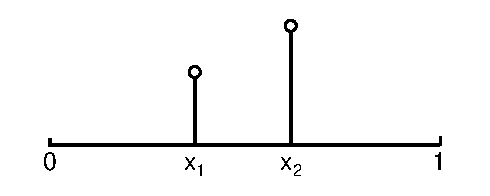
\epsfig{file=mi1.eps}}\end{center}
 
\begin{center}
Fig. 1
\end{center}
 \end{figure}
then there must be at least one local minimum somewhere in the
 range $0 < x < x_2$. Now in this new range, we already have one
 point $(x_1)$, so that a further  reduction in range is possible                                     
 with only one new function evaluation,                                     
  and the procedure can now be continued
with only one new evaluation per stage.
It remains to be shown that this can be continued indefinitely
with a constant reduction in step size, and to calculate what that
reduction will be. Clearly we would get the maximum reduction on the
first step if $x_1$ and $x_2$
were very close together, but we must not forget that
$x_1$ (or $x_2)$ will then be used for the next stage and should therefore be
close to the middle of this new interval as well.  The situation is
illustrated in the figs. 2 and 3, where the distances indicated are
imposed by the symmetry of the intervals and the condition that the
reduction in range must be a factor of $t$ in each stage.  The new range
after evaluation of $F(x_3)$ will be $x_3 < x < x_2$ and
its length must be~$t^{2}$.
 
\begin{figure}
\begin{center}\mbox{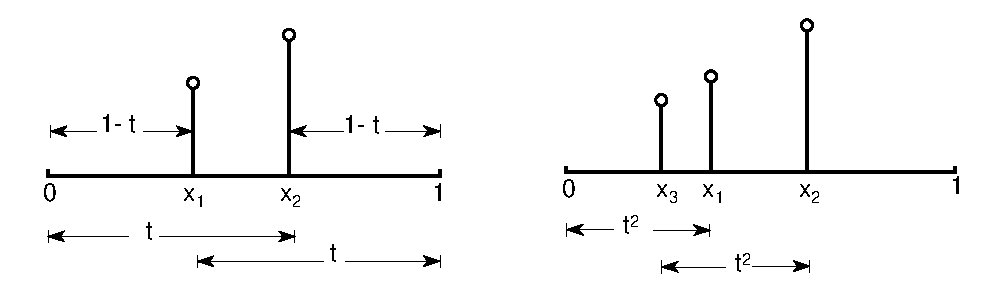
\epsfig{file=mi23.eps,width=.99\textwidth}}\end{center}
 
\begin{center}
Fig. 2\hskip68mm Fig. 3
\end{center}
 \end{figure}
 
This will be possible since there is a real root to the equation:
\begin{eqnarray}
t^2&=&1~-~t\nonumber\\
t&=&{\sqrt{5}~-~1\over
2}~\approx~0.616~.\nonumber
\end{eqnarray}                                  
 
 
Since this ratio $t$ is known as the {\em golden section}, the minimization
technique is called a golden section search.
If the number of stages
to be taken is known in advance, it is possible to improve very slightly
on this technique by using a {\em Fibonacci search}, as described for example
in Kowalik and Osborne \cite{Kowa}.  Although Fibonacci can be shown to be optimal
(in a sense described below), the slight improvement is probably not
worth the added complication.  The golden section search is optimal
among algorithms where the stopping point is not decided in advance.
 
     The above techniques are optimal only in the {\em minimax} sense, that is
they minimize the maximum number of function evaluations necessary to
obtain a given accuracy.  It might be called the pessimist's optimality, 
since in game theory it is the best strategy against an intelligent
opponent who is trying to make you lose.  It should therefore be
effective
in minimizing pathological functions, but in more normal cases we should
expect other methods to be better.  Such methods are described in the
following sections.
 
 
\section{Quadratic interpolation and extrapolation}
 
     A more optimistic approach consists in studying the expected
behaviour of the function and then hoping that the deviations of the
real function from this behaviour are not too great.  From the Taylor's
series analysis of Section 1.5, it would be reasonable to proceed by
assuming that the function is nearly quadratic.
 
     Since a parabola is determined by three points, this method requires
the function to have been evaluated for three different values $x_1, x_2$
and $x_3$. It then predicts the minimum to be at the minimum of the
parabola passing through these points.  If the three function values are
$F_1, F_2,$ and $F_3$, the predicted minimum is at $x_4$ given by
 $$x_4~=~\frac%
      {{\Tstm (x_2~+~x_3)F_1\over\Tstm (x_1~-~x_2)~(x_1~-~x_3)}
  ~+~  {\Tstm (x_1~+~x_3)F_2\over\Tstm (x_2~-~x_1)~(x_2~-~x_3)}
  ~+~  {\Tstm (x_1~+~x_2)F_3\over\Tstm (x_3~-~x_1)~(x_3~-~x_2)}}%
  {2~\left[    {\Tstm F1 \over \Tstm (x_1~+~x_2)~(x_1~-~x_3)}
           ~+~ {\Tstm F_2\over \Tstm (x_2~+~x_3)~(x_2~-~x_3)}
           ~+~ {\Tstm F_3\over \Tstm (x_3~+~x_1)~(x_3~-~x_2)}
    \right]}~. $$ 
Considerable simplification results when the three points are equally
spaced, a distance $d$ apart, in which case:
$$x_4~=~x_2~+~{d\over 2}~{(F_1~-~F_2)\over
(F_1~+~F_3~-~2F_2)}~.$$  
 The function is then evaluated at $x_4$, this point replaces one of the
first three, and a new point is predicted, again by quadratic
interpolation using the new set of three points.
The method terminates when the
predicted function value at some new point agrees with the actual value
within a specified tolerance.
 
     This algorithm usually performs quite well when applied to easy
(nearly quadratic) functions, but suffers from a number of instabilities
which can be quite serious, as follows:
 
  i) At any step the three points may determine a parabola with a maximum
     rather than a minimum, in which case the method diverges.
 
 ii) If the three points lie nearly in a straight line, the algorithm
     takes an enormous step which may cause numerical difficulties as
     well as diverging.
 
iii) After each step there is a choice of which two of the three previous
     points to retain for the next step.  It is usually more convenient
     and logical to retain the most recent points, but this may also lead
     to instabilities by throwing away the best points.
 
 iv) Even without any of the above difficulties, the method may oscillate
     about the minimum instead of converging toward it.
 
     All the problems can be fixed by including checks and safeguards in
the algorithm, but the remedies always involve abandoning, at least
temporarily, the quadratic interpolation step.
The best remedy is probably
to reserve the method for well-behaved functions and to abandon it
entirely as soon as trouble arises.  It is most often used as the last
step in algorithms which depend principally on other methods, since
physical functions are usually quite parabolic in the immediate
vicinity of the minimum.
 
     When derivatives of the function are available, variations of
quadratic interpolation are possible, using instead of three points to
determine the parabola, either two function values and one first
derivative, or the function value and the first two derivatives at one
point. These
variations tend to be even more unstable than the basic method, since
they use information from fewer points.
 
 
\Section{8cm}{The success-failure method}
 
     A good compromise between the stability of the grid search and the
rapid convergence of quadratic interpolation is found with the
success-failure
 technique of Rosenbrock \cite{Rose}.  A start point $x_0$ and initial step size
$d$ are required, and the function is evaluated at $x_0$ and $x_0 + d$.  The first
step is termed a success if $F(x_0 + d)< F(x_0)$, otherwise it is a failure. 
If it is a failure, $d$ is replaced by $-\beta d$, where $\beta$ is a contraction
factor less than one, and the test is repeated.  If it is a success, $x_0$ is
replaced by $x_{0} + d$, $d$ is replaced by $\alpha d$, where  $\alpha$ is an expansion factor
greater than one, and the test is repeated.  The process continues in
this way until the function values change by less than a specified amount,
The numerical values usually used for the expansion and contraction
parameters are $\alpha~\approx~3.0$ and $\beta~\approx~0.4.$
 
     An interesting feature of this method is that a local minimum is
always bracketed whenever a success is followed by a failure.  When this
happens, the middle one of the last three points is always lower than
the outer two, so that one is in a favourable position for trying a
quadratic
interpolation step.  The success-failure method, with one quadratic
interpolation step each time a success is followed by a failure, is
probably
the most effective one-dimensional technique for use on general functions
although in special cases other methods may be superior.
 
\chapter{Stepping Methods in many Variables}
\section{Grid searches and random searches}
 
   An excellent illustration of the enormous increase in complexity in
going to spaces of high dimensionality is afforded by the grid search
technique in many variables. In order to localize a minimum to 1\% of
the range of one variable by this technique requires 100 function
evaluations; in ten variables the number of points required is $10^{20}$.
Clearly we can forget about this method when more than one or
two parameters are involved.
 
In fact it is a general rule in function minimization, as in
function integration, that one should not expect good one-dimensional
techniques to be good when extended to higher dimensionality. Experience
with integration suggests that a {\em Monte Carlo search} is more efficient
than a grid search in many dimensions. The Monte Carlo technique
consists in
choosing points randomly according to some distribution
   (usually uniform or normal).
 
        But even when these methods are refined by using variable search
   ranges, they prove far too slow for general use and we must turn to more
   efficient techniques.
 
 \section{Single-parameter variation}
 
        Since the condition for a minimum which is a stationary point in
  $ n$ variables $x_i$ is the vanishing of all $n$ first derivatives
$\partial F/\partial x_i$, it is
   natural to try to make each derivative vanish separately, one after the
   other.  This is the old method of single
   parameter variation, where one seeks a
   minimum with respect to one\break\hfill
\begin{figure}[t]
\begin{minipage}[b]{.49\textwidth}
\begin{center}\mbox{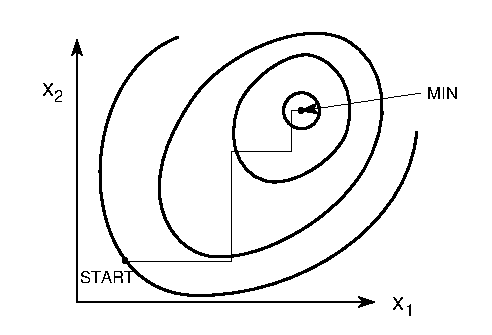
\epsfig{file=mi4.eps,width=.96\textwidth}}\\
Fig. 4
\end{center}
\end{minipage}  \hfill
\begin{minipage}[b]{.49\textwidth}
\begin{center}\mbox{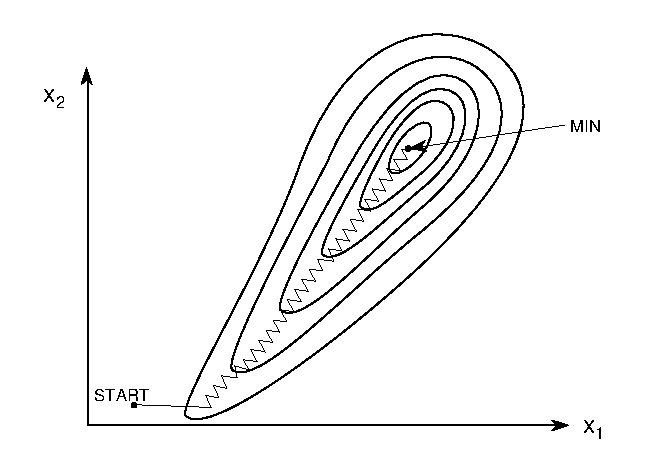
\epsfig{file=mi5.eps,width=.96\textwidth}}\\
Fig. 5
\end{center}
\end{minipage}
\end{figure}
\noindent
 variable at a time using one of the techniques described
 earlier.  Of course when you have finished
 minimizing with respect to $x_2$ you may no
longer be at a minimum with respect to $x_1$,
  so you generally have to start all over
 again, but the process usually does
 converge, as illustrated for two variables in
 fig. 4. Here the curves represent
contours of equal function value, and the straight lines show the steps
taken in minimizing $F$ with respect to $x_1$, then $x_2$, then $x_1$, etc.  In
this case the method converges nicely after only four single-parameter
minimizations.
 
     Consider now the function represented by the contours shown in fig. 5.
Here the method proceeds much more slowly because of the narrow valley. It still converges, but as
the valley becomes narrower, the convergence becomes arbitrarily slow.
 
Such behaviour in many dimensions causes this method to be generally
considered as unacceptably slow.
 
     Two of the more successful improvements aimed at avoiding such
behaviour are due to Hooke and Jeeves \cite{Hook} and Rosenbrock \cite{Rose}.  We discuss
the latter below.
 
 
\section{Rosenbrock's method}
 
     Rosenbrock's algorithm \cite{Rose} starts by performing single-parameter
minimizations as above.  Then when one full cycle of all parameters has
been completed, a new set of orthogonal axes is defined with one axis
taken as the vector from the start point to end point of the cycle.
This vector points in the direction of previous over-all improvement and
is expected to be a good direction for future improvement.  In the case
of the narrow valley seen above, it should point more or less along the
valley and avoid the zig-zag behaviour.  The next cycle of single-variable
 minimizations is performed using multiples of the newly defined
axes as variables.
 
     The Rosenbrock method generally performs well, being quite stable
and capable of following narrow valleys, but as the number of variables
increases, the efficiency drops, probably because the new axis defined
by past improvement is the only `intelligent direction' used in the next cycle. All the other
minimization directions are simply chosen orthogonal to the first one. Also, its terminal
convergence is slow compared with the more `quadratic' methods described in Section 4.
 
 
     Another technique, that of Davies, Swann, and Campey \cite{Dixo} (unpublished,
see Ref. 4) is similar to Rosenbrock's and will not be described here.
 
 
\section{The simplex method}
 
     One of the most successful stepping methods in many variables is
that of Nelder and Mead \cite{Neld}, based on the simplex.  A simplex is an 
$n$-dimensional figure specified by giving its $n$ + 1 vertices.  It is a
triangle in two dimensions, a tetrahedron in three, etc.  The algorithm
takes the name simplex because at each step the information it carries
about the function consists of its values at $n$ + 1 points.  One can
easily visualize how the method works by considering the
two-dimensional
case as in fig. 6.  The three starting simplex points are
somehow  chosen (perhaps randomly) and the function is evaluated at each
point.  Let the point $P_H$ be that at which the function value is highest
(worst) and $P_L$ that at which it is lowest. Let $\bar{P}$ be the centre-of-mass
of all points in the simplex except $P_H$;  that is:
 
 $$\bar{P}~=~{1\over n}\left\{\sum^{n+1}_{i=1}~P_i~-~P_H\right\}~.$$ 
\begin{figure}[t]
\begin{center}\mbox{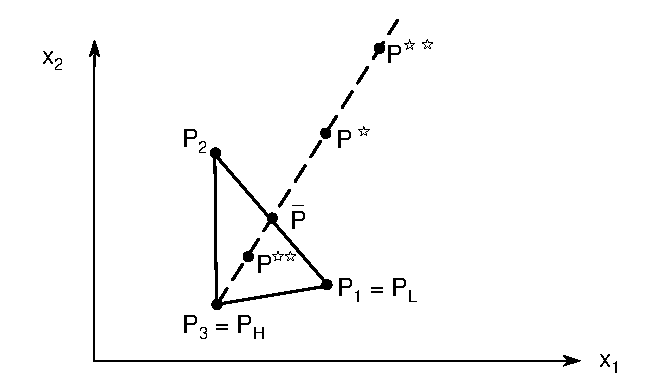
\epsfig{file=mi6.eps}}\end{center}
 
\begin{center}
Fig. 6
\end{center}
\end{figure}
\noindent
From the original simplex, a new simplex is formed by replacing $P_H$ by
a better point if possible.  The first attempt to find a better point is
made by reflecting $P_H$ with respect to $\bar{P}$, producing
$P^* = \bar{P} + (\bar{P} - P_H)$.
If $F(P^*) < F(P_L)$, a new point is tried at $P^{**} = \bar{P} + 2(\bar{P} - P_H)$.  If
$F(P^*) > F(P_H)$, a new point is tried at $P^{**} = \bar{P} - 1/2(\bar{P} - P_H)$.  The best of
the new points then replaces $P_H$ in the simplex for the next step, unless
none of them is better than $P_H$. In the latter case, a whole new simplex
is formed around $P_L$, with dimensions reduced by a factor of 0.5.
 
     Variations on the method are possible by using different contraction
or expansion factors when searching along the line from $P_H$ through $\bar{P}$
(dotted in diagram).  Another interesting possibility is to attempt a
quadratic interpolation step along the dotted line whenever three points
have been determined $(P_H, P^*, P^{**})$.  However, one must be careful not to
accept a point too close to $\bar{P}$, for then the simplex collapses into a line
(or in general a hyperplane of $n - 1$ dimensions) from which it can never
recover.
 
     The simplex algorithm, being designed always to take as big steps
as possible, is rather insensitive to shallow local minima or fine
structure in the function caused by rounding errors, statistical errors
(Monte Carlo output), etc.  Another of its virtues is that of requiring
few function evaluations, usually one or two per iteration.  In addition,
each search is in an `intelligent' direction, pointing from the highest
value to the average of the lowest values.  Compare this with Rosenbrock's
method, where really only the principal axis is an `intelligent' direction,
and all other searches are for exploring along orthogonal axes to
determine a new principal axis.
 
     A convenient convergence criterion for the simplex method is based
on the difference $F(P_H) - F(P_L)$.  The iterations are stopped when this
difference is less than a preset value.  As a final step, the function is
evaluated at $\bar{P}$, which is often slightly better than $F(P_L)$.
 
     In view of the danger mentioned above---of the simplex collapsing
into a hyperplane of dimension $n~-~1$---it has been suggested to use $n~+~2$
or more points rather than $n$ + 1 at each step.  I have tested this idea,
which is equivalent to introducing a dummy parameter of which the
function is independent, and have always found the efficiency of the
algorithm to decrease under these conditions.
 
\section{Conjugate directions method}
 
This method does not require information about the derivatives of the function, 
but the
exploration requires the material
developed in Chapter~\ref{sec:gradmeth}, so it is discussed in 
Section~\ref{sec:conjdir2}.
 
\chapter{Gradient Methods}
\label{sec:gradmeth}
 
\section{Calculating derivatives}
 
     I will call a {\em gradient method} any technique which uses information
from a very small range of the variables (i.e. essentially derivatives)
to predict good trial points relatively far away. This does not necessarily
 mean that they follow the gradient, but only that the gradient, and
perhaps higher derivatives, are used or estimated.
 
     It is of course possible in most cases to calculate analytically the
numerical values of the derivatives of a function, just as it is possible
to calculate the value of the function itseif.  However, it is often
inconvenient and dangerous if the algebra is complicated, so that very
often we are faced with minimizing a function for which no derivatives
are provided. Since the most powerful algorithms discussed below require
derivatives, a general minimization program must be able to estimate the
derivatives of the function by finite differences.
 
     A first derivative may be estimated from
$$\left .{\partial F\over \partial x}\right|_{x_{0}}~\approx~{F(x_0~+~d)~-~F(x_{0})\over
d}~,$$ where $d$ is a `small' displacement.  The error will be, to lowest
order in the Taylor's expansion,
$$\left .\delta~\approx~{d\over 2} \cdot {\partial^{2}F\over \partial x^{2}}\right|_{x_{0}}~.$$
 It is therefore advantageous to make $d$ as small as possible, but still
large enough so that the rounding error in the computation of $F$ does not
become larger than the error introduced by $\delta$. Since the second derivatives may not be known,
it may not be possible to find an optimum step-size $d$, so we may just have to close our eyes and
guess.
 
     A much safer method would be to use points chosen symmetrically
on either side of $x_0$ giving
 $$\left .{\partial F\over \partial x}\right|_{x_{0}}~\approx~{F(x_0~+~d)~-~F(x_0~-~d)\over
2d}~,$$ for in this case the error  $\delta$ vanishes to second order and the lowest
order term is proportional to the third derivative. A disadvantage of
this method is that it requires $2n$ function calls to estimate the $n$ first
derivatives, whereas the asymmetric steps require only $n$ + 1 [or only $n$ if
$F(x_0)$ has to be evaluated anyway].  An advantage of the symmetric steps
method, however, is that it gives the second derivatives as a
by-product [assuming $F(x_0)$ known]:
 
 $${\partial^{2} F\over \partial x^{2}}~\approx~{F(x_0~-~d)~+~F(x_0~+~d)~-~2F(x_{0})\over d^{2}}~,$$
and from the relationship for the error $\delta$ in the asymmetric method,
 a conservative upper limit of the uncertainty in the first derivative
results assuming at least that the symmetric formula gives a smaller
error than the asymmetric one.  A complete treatment of step sizes is
beyond the scope of these lectures but can be found in a paper by
Stewart \cite{Stew}.
 
     The numerical evaluation of second derivatives is facilitated by
the fact that they should be approximately constant over small regions,
so that symmetrical steps are usually not necessary.  Unfortunately,
however, there are a lot of second derivatives to evaluate;  since they
form a symmetric $n~\times~n$ matrix, there are $n(n + 1)/2$ independent
components, requiring at least $n(n - 1)/2$ points  in addition to those
 required for the symmetric derivatives.
\begin{figure}
\begin{minipage}[b]{.49\textwidth}
\begin{center}\mbox{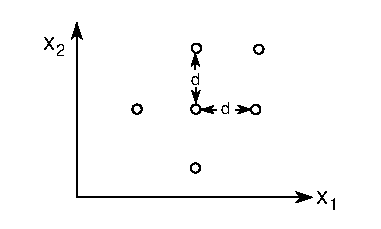
\epsfig{file=mi7.eps}}\\
Fig. 7
\end{center}
\end{minipage} \hfill
\begin{minipage}[b]{.49\textwidth}
\begin{center}\mbox{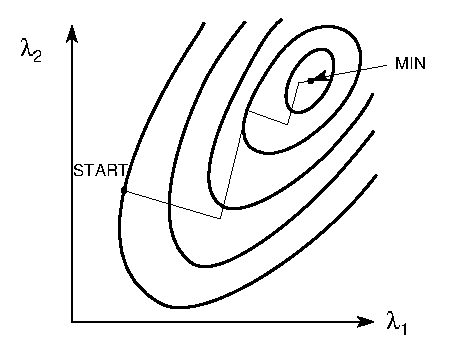
\epsfig{file=mi8.eps}}\\
Fig. 8
\end{center}
\end{minipage} \hfill
\end{figure}
 For two parameters, a minimum
  point pattern is shown fig. 7. The odd point (for
 the mixed second derivative) could
 have been chosen in any corner. The
 two-dimensional diagram is somewhat
 misleading since for large $n$, the
number of `odd points' is $n$ times
  larger than the number of `symmetric' points.
 
\section{Steepest descent}
 
     As soon as the function's first derivatives are known, it is natural
to follow the direction of the negative gradient vector in seeking a
minimum, since this is the direction in which the function is decreasing
the fastest.  Such a technique was used by Cauchy more than a century
ago, and is the basis of what is now known as the method of steepest
descent.
 
     This method consists of a series of one dimensional minimizations,
each one along the direction of local steepest descent (gradient) at the
point where each search begins.  Of course the direction of the gradient
is not constant along a line even for a general quadratic function, so
we expect many iterations to be necessary, but the method can be shown
to converge for a quadratic function. 
 Let us follow its progress
 for a typical function whose contours are shown
 in fig. 8.
   We immediately see an unfortunate
 property of the successive search
 directions: if each linear minimization is exact,
 successive searches must be in orthogonal
directions.  In two dimensions,
this yields steps which look just
like the single parameter variation method (fig. 5) with the axes rotated to
line up with the gradient at the start point.  In many dimensions the
situation is not quite so bad, but successive directions are still
orthogonal and the algorithm cannot be considered acceptable.
\begin{figure}
\begin{center}\mbox{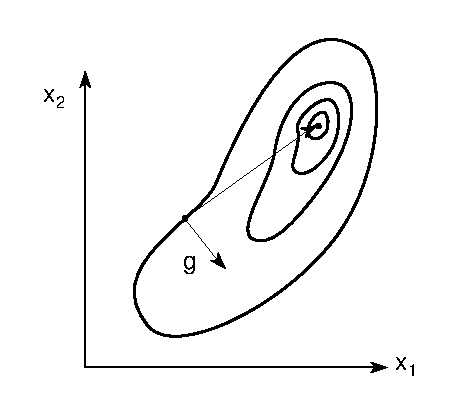
\epsfig{file=mi9.eps}}\end{center}
 
\begin{center}
Fig. 9
\end{center}
\end{figure}
     It is in fact easy to draw contours for a reasonably well-behaved
 hypothetical function (fig. 9)
 where the direction to the
 minimum is just perpendicular to the gradient.
 
\section{Newton's method}
 
     It is clear that since a general quadratic function is determined
by specifying its value, first derivatives, and second derivatives at a
point, it can be minimized in one step if and only if all this information
(or its equivalent) is taken into account.  Let us write a
quadratic function as
 $$F({\underline{x}})~=~F({\underline{x}}_0)~+~{\underline{g}}^T 
({\underline{x}}~-~{\underline{x}}_0)~+~{1\over 2}~({\underline{x}}~-~{\underline{x}}_0)^T~\UTG
   ({\underline{x}}~-~{\underline{x}}_0)~,$$
 where the gradient ${\underline{g}}$ is evaluated at ${\underline{x}}_0$ and the second derivative
matirx $\UTG$is a constant.  Then the minimum is given directly by
 
                     $${\underline{x}}_m~=~{\underline{x}}_0~-~\UTG\!\!^{-1}{\underline{g}}~=~
{\underline{x}}_0~-~\UTV{\underline{g}}~,$$
 where the inverse of the second derivative matrix is the {\em covariance
matrix} $\UTV$.
 
     This is then the many-dimensional equivalent of quadratic
interpolation
discussed earlier, and it is subject to the same sort of difficulties
when applied as an iterative technique to general non-quadratic functions.
But let us first point out its good features:
 
  i) the step size is no longer arbitrary, but is prescribed precisely by
     the method;
 
 ii) the step directions are no longer necessarily along the gradient
     vector but take account of parameter correlations (narrow valleys
     or ridges) through the mixed second derivative terms.
 
     In practice, however, the method is unstable, essentially for the
reasons given in Section 2.4.  In particular, it diverges whenever the
matrix $\UTG$ (or $\UTV$) is not positive-definite (see next section).  In its
unmodified form  the method is used only when the minimum is known to
be very close or when the function is known to be positive quadratic (for
linear least squares).  However, it is clearly a powerful technique
and is worth studying in some detail since all the most successful
algorithms are based on {\em Newton-like steps}, as discussed below.
 
\section{Positive-definite quadratic forms}
 
     We pause here briefly to consider the properties of quadratic forms
useful for understanding the more powerful gradient methods.  In one
dimension the description is simple;  a general quadratic form can be
written
  $$F(x)~=~a~+~gx~+~{1\over 2}~Gx^2~, $$
 where $g = \partial F/\partial x$ at $x$ = 0, and $G = \partial^2 F/\partial x^2$ also at $x$ = 0.
This function
has a minimum if and only if $G \ge$ 0.  If $G$ = 0, the minimum is at infinity,
The minimum (if it exists) is at $x = -g/G$.  When using a quadratic
approximation to minimize a general non-linear function, it makes sense to
take a step to $x = -g/G$ only if $G > 0$ since otherwise we step to
a predicted maximum or to infinity.  A possible remedy if $G < 0$ is to
take a
step $x = -g$;  that is, to set $G$ arbitrarily equal to unity so that the
step will at least be in the right direction although it will now have
arbitrary length.  Consideration of fig. 10 shows that this is
the only thing we can do unless more information is available, since the
quadratic part of the function is not {\em convex} or {\em positive-definite} at
the point $x_0$.
 
\begin{figure}
\begin{minipage}[b]{11cm}
\begin{center}\mbox{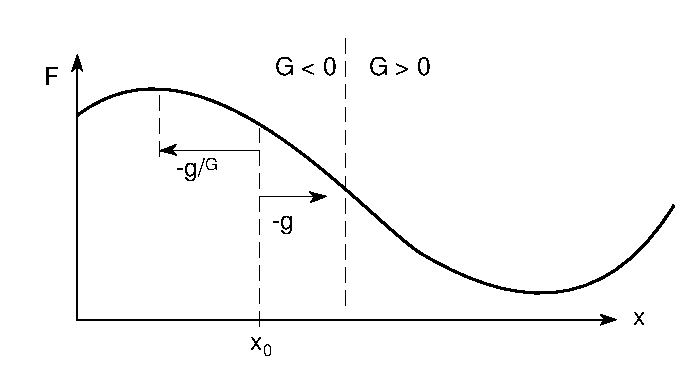
\epsfig{file=mi10.eps,width=108mm}}\\
Fig. 10
\end{center}
\end{minipage} \hfill
\begin{minipage}[b]{49mm}
\begin{center}\mbox{
\epsfig{file=mi11.eps,width=48mm}}\\[5mm]
Fig. 11
\end{center}
\end{minipage}
\end{figure}
      These arguments may now be extended to many dimensions where $g$
becomes the gradient vector ${\underline{g}}$, and $G$ becomes the second derivative matrix
$\UTG$. Then the Newton step to ${\underline{x}} = -\UTG\!\!^{-1}{\underline{g}}$ makes sense 
only if $\UTG$
 (hence $\UTG\!\!^{-1})$ is a positive-definite matrix, since only then does the quadratic form
 $$F({\underline{x}})~=~a~+~{\underline{g}}^T \cdot {\underline{x}}~+~{1\over 2}~{\underline{x}}^T
\UTV {\underline{x}}$$
have a minimum.  If $\UTG$ is singular, the predicted minimum (or maximum)
is not unique.
 
     Unfortunately there is no simple way of telling, in general, if a
matrix is positive-definite by inspecting individual components, but we
can at least state some of the many useful properties of such matrices.
Two necessary (but not sufficient) conditions for a (square, symmetric)
matrix to be positive-definite are:
 
  i) the diagonal elements must be positive (this is in fact sufficient
     for a 1 $\times$~1 matrix);
 
 ii) the off-diagonal elements must obey $G^2_{ij} < G_{ii}G{jj}~.$
 
[Properties (i) and (ii) together are sufficient for a 2 $\times$ 2 matrix.]
While the above conditions are easy to check, they are not in general
sufficient.  Some necessary {\em and} sufficient conditions are the following:
 
 iii) All the eigenvalues of the matrix are positive. This is generally
      a rather difficult calculation and is usually approximate.
 
 iv) The determinants of all the upper left square submatrices (formed
     as indicated in the diagram in fig. 11) are
     positive.  This is probably the easiest method.
 
  v) The scalar ${\underline{e}}^T \UTG{\underline{e}}$ is positive for all vectors
${\underline{e}}$  This is usually
     taken as the definition of a positive-definite matrix, and explains
     why a positive-definite matrix yields a quadratic form with a
     minimum:  the function increases in all directions from ${\underline{e}}~=~0$.
 
 vi) The inverse $\UTG\!\!^{-1} = \UTV$ is positive-definite.
 
     Now suppose that $\UTG\!\!^{-1}$ is calculated for a Newton  step and turns out
to be non-positive-definite.  In analogy to the one dimensional case we
would simply take $\UTG = \UTI$, the unit matrix, and the Newton step would
become a steepest-descent step of arbitrary length, which is probably
not so bad an idea and is in fact often done.  But we can do better by
trying to make a positive-definite matrix which is as `close' as possible
to the unacceptable $\UTG$. This is done as follows:
 The matrix $(\UTG + \lambda \UTI)^{-1}$ is
used instead of $\UTG\!\!^{-1}$, where $\lambda$ is greater
     than the largest negative eigenvalue of $\UTG\!.$  This requires a fair
     amount of calculation and so is not very convenient, but it is
     quite appealing since it amounts to taking a step which is intermediate between a Newton step
and a steepest-descent step (for
     large values of  $\lambda$ the step becomes short and in the direction of
     the gradient).
 
 If we are willing to calculate eigenvectors as well as eigenvalues, the
     non-positive-definiteness can be turned into an advantage, since the eigenvector
corresponding to a negative eigenvalue
     indicates a direction (or directions) in which the negative first
     derivative is {\em increasing} in magnitude rather than decreasing.  This
     suggests an especially fruitful direction for a
single-parameter-variation step which should not only lead to a good
decrease of the
     function value but should also lead more quickly to a region of
     positive-definiteness.
 
     Minimization methods based on variations of Newton's method as
suggested by the above considerations are usually called quasi-Newton
methods.  Many such algorithms have been published and some are quite
successful, but the field is still open for new ideas.
 
     The principal drawback of such techniques is the repeated evaluation
 and inversion of the second-derivative matrix.  The calculation of
the second derivatives usually requires a rather long time, proportional
to $n^2$, and the matrix inversion, although usually faster, increases with
$n$ like $n^3$.
 
     One of the most interesting results concerning quadratic forms is
the basis of a collection of related techniques described in the next
sections, which do not require explicit repeated evaluations of $\UTG$.
 
 
\section{Conjugate directions}
\label{sec:conjdir2}
 
     The vectors ${\underline{d}}_i$ and ${\underline{d}}_j$ are said to be {\em conjugate} with
respect to a positive-definite symmetric matrix $\UTA$ if
 
 $${\underline{d}}^T_i \UTA{\underline{d}}_j~=~0\qquad {\rm for}\qquad i \neq j~.$$
 
If $\UTA$ is the unit matrix $\UTI$, the conjugate vectors $\UTd$ would be orthogonal,
so conjugacy can be thought of as a generalization of orthogonality. A
set of $n$ conjugate vectors span an $n$-dimensional space, and any point
in the space can therefore be expressed as a linear combination of $n$
conjugate vectors.
 
     Although the matrix $\UTA$ does not uniquely define a set of conjugate
vectors, such a set can always be constructed by a procedure similar to
the Gram-Schmidt orthogonalization method.  Let us start for example
with an arbitrary vector ${\underline{d}}_1$.  Then the vector
 
 $${\underline{d}}_2~=~\UTA{\underline{d}}_1~-~{{\underline{d}}^T_1
\UTA\UTA{\underline{d}}_1\over {\underline{d}}^T_1 \UTA{\underline{d}}_1}~{\underline{d}}_1$$
can be seen to be conjugate to ${\underline{d}}_1$ since the product ${\underline{d}}^T_1 \UTA
{\underline{d}}_2$ vanishes
identically.  The process can then be continued in the same way to
construct a ${\underline{d}}_3$ which will be conjugate to both ${\underline{d}}_1$ and 
${\underline{d}}_2$,
and so forth up to ${\underline{d}}_n$.
 
     Such vectors become interesting for minimization problems when they
are conjugate with respect to the hessian (second derivative) matrix $\UTG$.
In this case a theorem of Fletcher and Reeves \cite{Flet1} states that a sequence
of linear minimizations in each of the $n$ conjugate directions will
minimize a general quadratic function of $n$ variables.  That this is true
can be seen quite easily as follows.  Let the quadratic function be
 $$F({\underline{x}})~=~F({\underline{0}})~+~{\underline{g}}^T {\underline{x}}~+~{1\over 2}~
{\underline{x}}^T \UTG\!{\underline{x}}$$
 and the $n$ directions $d_i$ be conjugate with respect to $\UTG$:
             $${\underline{d}}_i^T\UTG{\underline{d}}_j~=~0~,\qquad i\neq j~.$$
Then the vectors ${\underline{x}}$ and ${\underline{g}}$ can be expressed as linear combinations
\begin{eqnarray}
{\underline{x}}&=&\sum_{i}~y_i{\underline{d}}_i\nonumber \\
\nonumber\\
{\underline{g}}&=&\sum_{i}~c_i{\underline{d}}_i~,\nonumber
\end{eqnarray}
so that the general quadratic becomes
 $$F({\underline{x}})~=~F({\underline{0}})~+~\left(\sum_i~c_i{\underline{d}}^T_i\right)
\left(\sum_j~ y_j{\underline{d}}_j\right)~+~{1\over 2}~\left(\sum_i~y_i{\underline{d}}^T_i\right)
\UTV~\left(\sum_j~ y_j{\underline{d}}_j\right)~.$$
 Now  if the last term above is regrouped as a double sum, the terms with
 $i\neq j$  drop out because of the conjugacy condition, so that the whole
expression can be simplified as
 \begin{eqnarray}
F({\underline{x}})&=&F({\underline{0}})~+~\sum_i~\sum_j~c_i{\underline{d}}^T_i
{\underline{d}}_j y_j~+~{1\over
2}~\sum_{j}~y^2_j{\underline{d}}^T_j\UTG{\underline{d}}_j\nonumber\\
&=&F({\underline{0}})~+~\sum_j~\left(b_j y_j~+~b^{\prime}_j y^{2}_j\right)\nonumber
\end{eqnarray}
where
 $$b_j~=~\sum_i~c_i{\underline{d}}^T_i{\underline{d}}_j$$
 and
 $$b^{\prime}_j~=~{\underline{d}}^T_j \UTG{\underline{d}}_j$$
 are constants. By expressing the quadratic in terms of $y$ instead of $x$
we have separated it into a sum of independent one-parameter quadratic
functions.  A minimization with respect to $y_i$ (a linear minimization
along the direction ${\underline{d}}_i$) will therefore be independent of the minimizations
along the other conjugate directions, which demonstrates the validity
of the theorem.
 
     The above theorem tells us what is `wrong' with the
single-parameter-va\-ria\-tion method:  we should
be using conjugate directions rather than
simply orthogonal axes.  However, since the construction of conjugate
vectors seems to require knowledge of the hessian $\UTG$, this does not yet
help very much in practice, for if we knew $\UTG$ (and ${\underline{g}}$) we could minimize
a quadratic immediately by means of Newton's method, and would not need
to use $n$ linear minimizations.
 
     The usefulness of conjugate directions comes from the fact that
there are ways of determining such directions implicitly, without first
evaluating the entire hessian matrix $\UTG$.  Of course, by the time all $n$
conjugate directions are determined, by whatever method, information
equivalent to the matrix $\UTG$ must have been determined.  However, by that
time considerable minimization may already have been performed, as in
the method implied by the following theorem.
 
If ${\underline{x}}_0$ and ${\underline{x}}_1$ are minimum points in two parallel subspaces, then
the direction 
\begin{figure}
\begin{center}\mbox{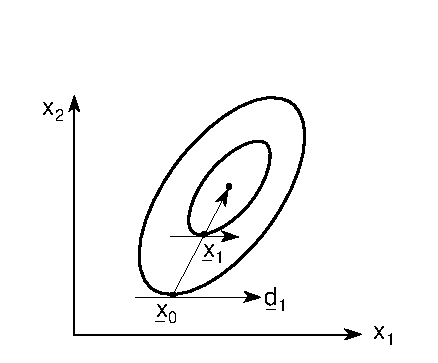
\epsfig{file=mi12.eps}}\end{center}
 
\begin{center}
Fig. 12
\end{center}
\end{figure}
${\underline{x}}_1-{\underline{x}}_0$
is conjugate to any vector which lies in either
 subspace. This can easily be seen in
two dimensions as illustrated
in  fig. 12. Since ${\underline{x}}_0$
 is a minimum along the direction ${\underline{d}}_1$
 the gradient of $F$ at ${\underline{x}}_0$ must be
 orthogonal to ${\underline{d}}_1$:
$${\underline{d}}^T_1({\underline{g}}~+~\UTG
{\underline{x}}_0)~=~0~,$$ 
where ${\underline{g}}$ is the gradient at ${\underline{x}} = {\underline{0}}$.  
Similarly at ${\underline{x}}_1$:
$${\underline{d}}^T_1({\underline{g}}~+~\UTG
{\underline{x}}_1)~=~0~.$$
Subtracting the above equations, the first terms drop out and we have:
 $${\underline{d}}^T_1 \UTG({\underline{x}}_1~-~{\underline{x}}_0)~=~0~,$$
showing that $({\underline{x}}_1~-~{\underline{x}}_0)$ is conjugate to ${\underline{d}}_1$.
 
     Unfortunately, extending this algorithm to three dimensions requires
three additional minimizations in order that the third direction be
conjugate to both of the first two, so that convergence for a general
quadratic in $n$ variables is obtained only after $n$ iterations involving in
all $n(n$ + 1)/2 linear minimizations.  Since this is just the number of
independent elements in the second derivative matrix, we would be better
off for quadratic functions to calculate this matrix directly and avoid
the linear searches.  On the other hand, for non-quadratic functions the
conjugate directions method should be much more stable since it proceeds
by a series of linear searches in independent directions and still
guarantees convergence in a finite number of steps once a quadratic
region is entered.  In addition, this method has the advantage of
requiring neither first nor second derivatives of the function.
(Strictly speaking, then, it should have been discussed in Section 3
rather than in this section.)
 
      A disadvantage of the algorithm described above is that for each
iteration, $n$ minimizations are performed in direction ${\underline{d}}_1$, whilst only
one is performed in direction ${\underline{d}}_n$.  This undesirable asymmetry is largely
avoided in a variation due to Powell \cite{Powe1}.
 
\section{Conjugate gradients}
 
      When the first derivatives of the function are calculated, a somewhat
more elegant method can be used, known as the method of {\em conjugate
gradients} \cite{Flet1}. Suppose that the function and its gradient are evaluated
at two points ${\underline{x}}_0$ and ${\underline{x}}_1$, giving differences:
 \begin{eqnarray}
{\underline{\Delta}}{\underline{x}}&=&{\underline{x}}_1~-~{\underline{x}}_0\nonumber\\
{\underline{\Delta}}{\underline{g}}&=&{\underline{g}}_1~-~{\underline{g}}_0~.\nonumber
\end{eqnarray}
Then if the function were quadratic with hessian $\UTV$ we would have
 $${\underline{\Delta}}{\underline{g}}~=~\UTG~ {\underline{\Delta}}{\underline{x}}~.$$
Any vector ${\underline{d}}_1$ orthogonal to ${\underline{\Delta}}{\underline{g}}$
 would then be conjugate to ${\underline{\Delta}}{\underline{x}}$:
 $${\underline{d}}^T_1~{\underline{\Delta}}{\underline{g}}~=~
{\underline{d}}^T_1~\UTG~{\underline{\Delta}}{\underline{x}}~=~0~,$$
 which immediately suggests a method for obtaining conjugate directions
without knowing $\UTG$, based on the change in gradient along a previous
direction.
 
     In the method of conjugate gradients, successive one-dimensional
minimizations are performed along conjugate directions with each direction being used only once per iteration.  The first direction is taken
as ${\underline{d}}_0 = -{\underline{g}}_0$, the steepest descent vector at ${\underline{x}}_0$. 
Let the minimum along this direction be at ${\underline{x}}_1$ where the gradient is
${\underline{g}}_1$.  Then the next  search direction ${\underline{d}}_1$, which we want to be
conjugate to ${\underline{d}}_0$ must be a linear combination of the only vectors we have at hand,
namely:
 $${\underline{d}}_1~=~-{\underline{g}}_1~+~b{\underline{d}}_0~.$$
The conjugacy condition is
 $${\underline{d}}_1^T\UTG{\underline{d}}_0~=~{\underline{d}}_1^T\UTG({\underline{x}}_1~-~
{\underline{x}}_0)~=~0$$
or
$$(-{\underline{g}}_1^T~+~b{\underline{d}}_0^T)\UTG{\underline{d}}_0~=~
(-{\underline{g}}_1^T~-~b{\underline{g}}_0^T)({\underline{g}}_1~-~{\underline{g}}_0)~=~0~.$$
Since ${\underline{x}}_1$ is a minimum along direction ${\underline{d}}_0 = -{\underline{g}}_0$, the
direction ${\underline{g}}_0$ is orthogonal to the gradient at ${\underline{x}}_1$,
 so that ${\underline{g}}_1^T{\underline{g}}_0 = 0$.  We are then left with
 $$b~=~{{\underline{g}}_1^T{\underline{g}}_1\over {\underline{g}}_0^T{\underline{g}}_0}$$
 so that the new conjugate direction is
 $${\underline{d}}_1~=~-{\underline{g}}_1~+~\left(
{{\underline{g}}_1^T{\underline{g}}_1\over {\underline{g}}_0^T{\underline{g}}_0}\right)~
{\underline{d}}_0~.$$ 
This process can be continued to generate $n$ directions, each one conjugate
to all the others.  It turns out that the same simple formula holds
for all the successive conjugate directions
 $${\underline{d}}_{i+1}~=~-{\underline{g}}_{i+1}~+~\left(
{{\underline{g}}_{i+1}^T{\underline{g}}_{i+1}\over {\underline{g}}_i^T{\underline{g}}_i}\right)~
{\underline{d}}_i~.$$ 
 
\section{Variable metric methods (VMM)}
 
     In analogy with the methods of differential geometry and general
relativity, it is convenient to consider the properties of the function
$F({\underline{x}})$ as being in fact properties of the space of the variables ${\underline{x}}$.
 We have already made some rudimentary use of this idea when we generalized
from the usual orthogonal coordinate axes to a system defined by axes
pointing in conjugate directions.  We now wish to go further and be able
to express the properties of the function $F$ geometrically as the properties 
of the non-Euclidean space of its variables ${\underline{x}}$.
 
     The fundamental invariant in a non-Euclidean space is the squared
distance element
 $$ds^{2}~=~{\underline{d}}{\underline{x}}^T\UTA{\underline{d}}{\underline{x}}~,$$
 where ${\underline{d}}{\underline{x}}$ is a differential coordinate displacement and $\UTA$ is
the {\em covariant
metric tensor} which determines all the properties of the space under
consideration. When $\UTA$ is just the unit matrix $\UTI$, the above formula for
$ds^2$ just expresses the Pythagorean theorem for an $n$-dimensional
Euclidean
space. When off-diagonal elements of $\UTA$ are non-zero and when the
elements are allowed to vary as functions of ${\underline{x}}$, a generalized
non-Euclidean space is generated.
 
     It is easily verified that the second derivative (hessian) matrix $\UTG$
behaves under coordinate transformations like a covariant tensor and
we will identify it with the metric tensor of our space.  The inverse
$\UTV = \UTG\!\!^{-1}$ is a contravariant tensor and becomes the contravariant metric
tensor.  (For a discussion of covariant and contravariant tensors, see
for example chapter 10 of Ref. [9].)  This immediately enables us to
construct two scalar (invariant under coordinate transformations)
quantities:
$$a)\qquad ds^2~=~ {\underline{d}}{\underline{x}}^T\UTG{\underline{d}}{\underline{x}}$$
is the square of the generalized distance between the point ${\underline{x}}$ and the
point ${\underline{x}} + {\underline{d}}{\underline{x}}$.  When $F$ is a chisquare
 function which is minimized to
determine some best parameters ${\underline{x}}$, then the physical meaning of the
generalized distance $ds$ is just the number of `standard deviations'
 ${\underline{x}} + {\underline{d}}{\underline{x}}$ is away from ${\underline{x}}$.  
That is, the use of the metric tensor $\UTV$
enables
us to scale the distance ${\underline{d}}{\underline{x}}$ so that it comes out as a physically (or
statistically) meaningful invariant quantity instead of being expressed
in arbitrary units (or a mixture of arbitrary units!).
\vskip2mm \noindent
And{\phantom{xxxxxxxxxxxxxxxxxxx}} $b)\qquad \rho~=~{\underline{g}}^T\UTV{\underline{g}}$\\
\vskip2mm
\noindent
 is twice the difference between the function value at the point where $\UTV$
and the gradient ${\underline{g}}$ are calculated and the minimum of a quadratic form
with hessian matrix  $\UTG = \UTV\!\!^{-1}$.  That is, $\rho$/2 is the expected (vertical)
distance to the minimum if the function $F$ were quadratic. This provides
us with an important scale-free {\em convergence criterion} for any method
which provides approximations to $\UTV$ and ${\underline{g}}$.
 
     When the function $F$ is quadratic, $\UTG$ is constant everywhere and, in
the sense outlined above, this is equivalent to working in a space with
a constant metric.  For real non-linear functions we expect higher-order
terms to be small but not negligible, so that we can think of working in
a space with a slowly-varying metric tensor. Minimization methods based
on this approach are known as {\em variable metric methods}.  They differ from
the basic Newton-Raphson method in that the matrix $\UTG$ is not
completely
re-evaluated at each iteration, but is assumed to be well approximated by
taking the $\UTG$ of the previous iteration and applying a correction based on
new information from the current iteration.  This correction is known as
the {\em matrix updating formula}, which in general differs from method to
method.
 
     Variable metric methods therefore proceed generally by the following
steps:
 
  i) A starting point ${\underline{x}}_0$ is given, the gradient ${\underline{g}}_0$ at that point is
     calculated, and some approximation to  $\UTG\!\!^{-1}$, say $\UTV\!\!_0$, is constructed.
     The starting $\UTV\!\!_0$ may be only the unit matrix, or it may actually be
     the inverse of the full second derivative matrix.
 
 ii) A step is taken to ${\underline{x}}_1 = {\underline{x}}_0 - \UTV\!\!_0
{\underline{g}}_0$, which would be the
minimum if $F$
     were quadratic and if $\UTV\!\!_0$ were the true covariance matrix.  Since ${\underline{x}}_1$
     is not the position of the minimum in the general case, it is usual
     to perform a linear search along this direction, finding the $\alpha$
     which minimizes $F({\underline{x}}_0 - \alpha\UTV{\underline{g}}_0)$.  In either case let the
new point be
     called ${\underline{x}}_1$ and let the gradient calculated at ${\underline{x}}_1$ 
be ${\underline{g}}_1$.
 
iii) The matrix $\UTV$ is corrected using an updating formula of the form
 $$\UTV\!\!_1~=~\UTV\!\!_0~+~\UTf(\UTV\!\!_0,{\underline{x}}_0,
{\underline{x}}_1,{\underline{g}}_0, {\underline{g}}_1)~.$$
     Then ${\underline{g}}_0$ is replaced by ${\underline{g}}_1,~ {\underline{x}}_0$ by
${\underline{x}}_1$, and $\UTV\!\!_0$ by $\UTV\!\!_1$, and steps (ii)
     and (iii) are repeated until some convergence criteria are satisfied.
 
     The different methods differ chiefly in the choice of updating
function $\UTf$, as described in the following sections, and in the extent to
which linear minimizations are necessary.  Less important variations
involve the starting approximation $\UTV\!\!_0$ and various safeguards against
`unreasonable' steps and non-positive-definiteness as for the Newton
techniques.
 
 
\section{Davidon's rank-two formula}
 
     Probably the first---and perhaps still the best---variable metric
method was developed in 1959 by Davidon and later published in simplified
form in 1963 by Fletcher and Powell \cite{Flet}.  Davidon's updating formula for
the covariance matrix is the following:
 
$$\UTV\!\!_1~=~\UTV\!\!_0~+~{{\underline{\delta}}{\underline{\delta}}^T\over {\underline{\delta}}^T
{\underline{\gamma}}}~-~{~\UTV\!\!_0{\underline{\gamma}}{\underline{\gamma}}^T~\UTV\!\!_0\over
 {\underline{\gamma}}^T\UTV\!\!_0{\underline{\gamma}}}~,$$
where the changes in position and gradient on the last step were
 $${\underline{\delta}}~=~{\underline{x}}_1~-~{\underline{x}}_0$$
and
$${\underline{\gamma}}~=~{\underline{g}}_1~-~{\underline{g}}_0~,$$
 and $\UTV\!\!_0$ was the previous estimate of the covariance matrix.  This is
called a rank-two formula since the correction $\UTV\!\!_1 - \UTV\!\!_0$ is a matrix of
rank two in the space of $\delta$ and $\UTV\!\!_0{\underline{\gamma}}$ as can be seen directly by
inspection of the formula.
 
     One fundamental requirement of an updating formula is that the new
matrix satisfies the relationship
 $$\UTV\!\!_1{\underline{\gamma}}~=~{\underline{\delta}}~,$$
since ${\underline{\gamma}}~=~\UTG{\underline{\delta}}$ for a quadratic with hessian $\UTG$. 
 It is easily seen that Davidon's formula satisfies this requirement:
\begin{eqnarray}
\UTV\!\!_1{\underline{\gamma}}&=&\left[\UTV\!\!_0~+~{\delta\delta^T\over \delta^T\gamma}~-~
{\UTV\!\!_0{\underline{\gamma}}{\underline{\gamma}}^T\UTV\!\!_0\over {\underline{\gamma}}^T 
\UTV\!\!_0{\underline{\gamma}}}\right]~{\underline{\gamma}}\nonumber \\
&=&\UTV\!\!_0{\underline{\gamma}}~+~{{\underline{\delta}}{\underline{\delta}}^T{\underline{\gamma}}
\over {\underline{\delta}}^T{\underline{\gamma}}}~-~
{\UTV\!\!_0{\underline{\gamma}}{\underline{\gamma}}^T\UTV\!\!_0{\underline{\gamma}}\over
{\underline{\gamma}}^T\UTV\!\!_0{\underline{\gamma}}}\nonumber \\
&=&\UTV\!\!_0{\underline{\gamma}}~+~
{\underline{\delta}}~-~\UTV\!\!_0{\underline{\gamma}}~=~
{\underline{\delta}}~.\nonumber
\end{eqnarray}
 
  An unfortunate feature of the Davidon algorithm is the need to
perform at each iteration a linear minimization along the direction
given by a Newton step, $-\UTV{\underline{g}}.$  This linear search step is, however,
necessary in order to assure convergence for general functions. Fletcher
and Powell show \cite{Flet} that if the starting approximation to $\UTV$ is
positive-definite, then
$\UTV$ will remain positive-definite after all updatings, but
they have to use the fact that each iteration is a linear minimization,
that is
$${\underline{g}}^T_1\UTV\!\!_0{\underline{g}}_0~=~0~.$$
 
     It can be shown that this method is quadratically convergent, at
most $n$ iterations ($n$ linear searches and $n$ gradient calculations) being
required for an $n$-dimensional quadratic form.
 
 
\section{The rank-one formula}
 
     In an effort to avoid the linear minimizations required by Davidon's
algorithm, several workers have independently developed an interesting
updating formula of rank one.  In this case Davidon in 1968 was the
first
to publish an algorithm \cite{Davi} based on the formula, and Powell \cite{Powe2} has
summarized the properties of this formula and of algorithms based on it
 
     The rank-one updating is:
$$\UTV\!\!_1~=~\UTV\!\!_0~+~{({\underline{\delta}}~-~\UTV\!\!_0{\underline{\gamma}})
({\underline{\delta}}~-~\UTV\!\!_0{\underline{\gamma}})^T\over
{\underline{\gamma}}^T({\underline{\delta}}~-~\UTV\!\!_0{\underline{\gamma}})}~.$$
It can be shown \cite{Powe2} that this is the only formula of rank two (or less)
for which not only $\UTV\!\!_1{\underline{\gamma}} = \delta$ but:
$$\UTV\!\!_1{\underline{\gamma}}_i~=~{\underline{\delta}}_i~,$$
 where ${\underline{\delta}}_i$ and ${\underline{\gamma}}_i$ are the step
 and gradient changes at {\em any} previous
iteration.  This is known as the {\em hereditary property}, since $\UTV\!\!_1$ can be
said to
inherit the fundamental property $\UTV{\underline{\gamma}} = {\underline{\delta}}$  with respect
to all previous iterations (up to $n$).
 
     The hereditary property assures that after $n$ iterations, $\UTV\!\!_1$ will be
the true covariance matrix if $F$ is quadratic, no matter what steps were
taken (almost), so that if Newton steps are taken, convergence for a
quadratic function is assured after $n$ iterations, without the need for
linear minimizations.
 
     In addition, the rank-one formula is {\em symmetric}, in the sense that
the expression for $\UTV\!\!_1^{-1}$ in terms of $\UTV\!\!_0^{-1}$ is the same as that for
$\UTV\!\!_1$ in terms of $\UTV\!\!_0$ provided ${\underline{\delta}}$ and ${\underline{\gamma}}$ are
interchanged. The meaning of this symmetry property will be discussed in the next section.
 
     But, as nothing is perfect, so the elegance and mathematical beauty
of the rank-one formula hide a number of numerical and practical difficulties which can make it highly unstable when applied to a general
function.  In particular, if the vector ${\underline{\gamma}}$ happens to be orthogonal to the
vector $({\underline{\delta}}- \UTV\!\!_0{\underline{\gamma}})$, the denominator goes to zero in
the updating formula, and an unbounded correction is possible.  Since these vectors may be
orthogonal, even for a quadratic function, the problem of numerical
instability is a serious one.
 
     Moreover, the matrices $\UTV\!\!_1$ do not really converge to the true covariance matrix 
in the usual meaning of the term convergence.  Although
it is true that $\UTV\!\!_1$ will be equal to the true covariance matrix at the
$n^{\rm th}$ step for a quadratic function (barring numerical difficulties), the
intermediate matrices $\UTV$ may vary wildly from step to step, so that on
any particular iteration $\UTV\!\!_1$ may be a rather poor approximation.  This is
especially dangerous when the function is not quadratic, since the large
corrections necessary in later iterations will generally not compensate
properly the fluctuations in early steps.  Also, there is no guarantee
that intermediate matrices will remain positive-definite, and hence no
guarantee of a reduction in the value of $F$ at each step, even for a
quadratic $F$.
 
     All these difficulties can, of course, be overcome by programming
enough safeguards into the algorithm, but this can only be done at the
expense of efficiency and sometimes only by abandoning temporarily the
updating formula itself, which makes it lose some of its appeal.\\ \noindent
Different approaches are possible depending on whether it is considered
important to maintain positive definiteness as in the Davidon
algorithm \cite{Davi}, or important not to abandon the exact rank-one formula
as in Powell's method \cite{Powe2}.
 
 
\section{Fletcher's unified approach to VMM}
 
     The existence of two different updating formulas with very different
properties generated a lot of interest in variable metric methods (VMM)
during the years 1967--1971, since it showed VMM to be very promising
and left many questions unanswered, such as:
 
  i) How can it be that the rank-one and rank-two formulas have such
     different properties?  What is the relationship between them?
 
 ii) Is there a way to combine the best properties of both formulas?
 
iii) Are there other good formulas?  Is it possible to define a class
     of `admissible' formulas?
 
     A certain understanding of the above problems has recently been
made possible by the work of a number of people. In particular, a 
paper by Fletcher \cite{Flet2} presents a unified approach to VMM, which will be
given here.
 
     Recall that the rank-one equation is symmetrical (in a sense defined
in Section 4.9), but as we shall now see, the rank-two formula is not.
Indeed the asymmetry suggests a way to construct a possible third
formula
by taking the `mirror image' of the rank-two formula.  The basic idea is
that a new formula should satisfy the fundamental relationship
 $$\UTV\!\!_1{\underline{\gamma}}~=~{\underline{\delta}}~,$$
 and therefore its inverse should satisfy
 $${\underline{\gamma}}~=~\UTV\!\!_1^{-1}{\underline{\delta}}~.$$
 We can indeed write down the updating formula for $\UTV\!\!_1^{-1}$ which
corresponds to the rank-two formula for $\UTV\!\!_1$:
 $$\UTV\!\!_1^{-1}~=~\left(\UTI~-~{{\underline{\gamma}} {\underline{\delta}}^T\over
{\underline{\delta}}^T{\underline{\gamma}}}\right)
\UTV\!\!_0^{-1}~\left(\UTI~-~{{\underline{\delta}} {\underline{\gamma}}^T\over
{\underline{\delta}}^T{\underline{\gamma}}}\right)~+~
{{\underline{\gamma}}{\underline{\gamma}}^T\over
{\underline{\delta}}^T{\underline{\gamma}}}~.$$
This matrix $\UTV\!\!_1^{-1}$ can now be thought of as a mapping
from  ${\underline{\delta}}~\to~{\underline{\gamma}}$ since ${\underline{\gamma}} = \UTV\!\!_1^{-1}
{\underline{\delta}}$.  If we interchange ${\underline{\gamma}}$ and ${\underline{\delta}}$ 
in the formula, it
will then give a mapping from ${\underline{\gamma}} \to {\underline{\delta}}$, thereby
 producing a new updating formula
where $\UTV\!\!_1{\underline{\gamma}} = {\underline{\delta}}$.  The new {\em dual
 formula} will be just
 $$\UTV\!\!_1~=~\left(\UTI~-~{{\underline{\delta}}{\underline{\gamma}}^T\over
{\underline{\delta}}^T{\underline{\gamma}}}\right)\UTV\!\!_0
\left(\UTI~-~{{\underline{\gamma}}{\underline{\delta}}^T\over
{\underline{\delta}}^T{\underline{\gamma}}}\right)~+~
{{\underline{\delta}}{\underline{\delta}}^T\over {\underline{\delta}}^T{\underline{\gamma}}}~.$$
If we try this trick with the rank-one
formula, we just get the same rank-one formula back again, since it is symmetric in this sense, or
dual to itself.  But with the rank-two formula, the process of inverting
and interchanging yields a new formula, also of rank-two, which is also
a valid updating formula in the sense that it gives rise to a quadratically convergent VMM
algorithm.
 
     Now we go further and consider the class of formulas which includes
both rank-two and dual formulas as special cases.  Let us introduce the
notation
                   $${\phantom{xxxxx}}\UTV\!\!_1~=~\UTT(\UTV\!\!_0)\qquad   {\rm
for~the~rank-two~formula}~,$$ and
                   $$\UTV\!\!_1~=~\UTD(\UTV\!\!_0)\qquad   {\rm for~the~dual~formula}~,$$
 and consider the class of updating expressions as introduced by
Fletcher \cite{Flet2}:
 
$$\UTV_{\phi}~=~(1~-~\phi)\UTT~+~\phi(\UTD)~,$$
 where  $\phi$ is some parameter which determines the exact formula.  [Broyden \cite{Broy},
using a somewhat different notation, has also considered the same class
of formulas.]
 
     It then turns out that the rank-one formula is also in this class,
 with
 $$\phi({\rm rank-one)}~=~{{\underline{\delta}}^T{\underline{\gamma}}\over
({\underline{\delta}}^T{\underline{\gamma}}~-~
{\underline{\gamma}}^T\UTV\!\!_0{\underline{\gamma}})}~.$$
 
     Having now constructed a wide class of updating formulas, which in
fact includes all formulas known to the author, it will prove interesting
to consider their properties as a function of the generating parameter $\phi$.
Probably the most important property, and the only one we will consider
here, is that of {\em monotonic convergence} of $\UTV$ toward the true covariance
matrix for a quadratic function.  [This is called Property 1 in Fletcher's
paper \cite{Flet2} which should be consulted for details of the definition and for
theorems concerning it.]  The use of an updating formula with this
property will guarantee an improvement in the approximation $\UTV$ at each
iteration (for a quadratic function).
 
     Any formula $\UTV_{\phi}$ with $\phi$ in the interval [0,1] possesses the {\em monotonic}
convergence property.  Such a formula is said to belong to the {\em convex
class of formulas}. For any $\UTV_{\phi}$ with  outside the range [0,1], there
exists some quadratic function for which $\UTV$ diverges from the true
covariance matrix.
 
     From what we have already seen about the rank-one formula, it is
not surprising to find that it does not belong to the convex class.
Since  ${\underline{\delta}}^T{\underline{\gamma}} > 0$ for any step which is an improvement, 
and since ${\underline{\gamma}}^T\UTV\!\!_0{\underline{\gamma}} > 0$
if $\UTV\!\!_0$ is positive-definite, it can be seen immediately from inspection
of the equation for $\phi$(rank-one) that it must either be less than zero
or greater than one.
 
     The above considerations lead Fletcher to propose a new algorithm \cite{Flet2}
which is probably the most elegant and powerful of any VMM algorithm. 
Basically, he uses the general updating formula $\UTV_{\phi}$, with the value of $\phi$
chosen according to the following scheme:  If $\phi$(rank-one) $< 0$, set $\phi$ = 0,
corresponding to the usual  rank-two formula.  If $\phi$(rank-one) $> 1$, set
$\phi = 1$, corresponding to the dual formula. In this way, one always uses
a formula in the convex class, and chooses that one which is `closest'
to the rank-one formula.  It seems that the linear searches can then be
eliminated and replaced simply by Newton's steps, unless the function
is highly non-quadratic.  The latter condition can easily be detected by
comparing the actual improvement with the expected improvement at
each iteration.
 
 
\chapter{Specialized Techniques}
 
     All the methods outlined so far in these lectures are of rather
general applicability, the only assumption being---for some methods---a
 predominantly quadratic behaviour in the immediate vicinity of the
minimum. In order to develop more powerful methods than those already
presented, we will have to give up some of this generality and exploit
particular features of the functions to be minimized. In this section
we discuss a few specialized techniques which are still of rather wide
applicability in the sense that most functions of physical interest
fall in one or more of these classes.
 
\section{Chisquare minimization}
 
     Probably the most common application of minimization in scientific
research is in least squares fitting, where the function to be minimized
is the sum of squares of deviations, between measured values and predictions of 
a model containing variable parameters:
$$ 
F({\underline{x}})~=~\sum^{K}_{k=1}~f^2_k ({\underline{x}})~=~\sum^{K}_{k=1}~
\left({Y_k~-~T_k ({\underline{x}})\over \sigma_k}\right)^2~,$$
 where $Y_k$ and $\sigma_k $ are measured values and errors, and $T_k({\underline{x}})$ are the
values predicted by the model, depending on some parameters ${\underline{x}}$.
Minimizing $F$
then yields best values (estimates) of the $n$ parameters ${\underline{x}}$, based on $ K$
measurements ${\underline{Y}}$ with random errors $\sigma$, where $K$ must be greater than or
equal to $n$, and is usually much greater than $n$.
 
     Let us now consider the second derivative matrix for $F({\underline{x}})$, expressed
in terms of the individual $f_k({\underline{x}})$:
 
\begin{eqnarray}
{\partial^2F\over \partial x_i\partial x_j}&=&{\partial\over \partial x_i}~
{\partial\over \partial x_j}~\sum_k~f^2_k\nonumber \\
&=&{\partial\over \partial x_i}~\sum_k~2f_k~{\partial f_k\over \partial x_j}\nonumber \\
&=&\sum_k~2~ {\partial f_k\over \partial x_i}
~{\partial f_k\over \partial x_j}
~+~\sum_k~2f_k~{\partial^2f_k\over \partial x_i \partial x_j}~. \nonumber
\end{eqnarray}
 
In the above r.h.s., it is usual to make the approximation that the
second sum, involving second derivatives, is small compared with the
first term involving products of first derivatives.  This is called
{\em linearization}.  [Note that it is the {\em model}  $T({\underline{x}})$ that is being
linearized, not the function $F({\underline{x}}).$]  In the important special case of {\em linear
least squares}, the second sum is exactly zero, so that $F({\underline{x}})$ is quadratic, and
the whole minimization problem reduces to the inversion of the above
matrix $\partial^2F/\partial x_i \partial x_j$ (i.e. the taking of one Newton step).
 
 
     In the more general case of {\em non-linear least squares}, the
linearization approximation consists in taking
 
$${\partial^2F\over \partial x_i\partial x_j}~\approx~\sum_k~2~{\partial f_k\over \partial x_i}
~{\partial f_k\over \partial x_j}~.$$
 
This has the advantage of being easy to calculate and, moreover, it is
always positive-definite (under rather weak conditions such as the
existence of the derivatives, and provided it is non-singular). In fact
in many cases the use of the above approximation in computing Newton
steps is actually more effective than using the exact second derivative
matrix because of the positive definiteness.  Of course it must be
remembered that the covariance matrix obtained by inverting this
approximate
matrix does not in general converge to the true covariance matrix
even though the minimization  based on it may converge to the true
minimum.
 
\section{Likelihood maximization}
 
     An increasingly important alternative to the least squares method
in data fitting is the method of maximum likelihood.  In this case the
function to be minimized is of the form
 $$F({\underline{x}})~=~-\sum^{k}_{k=1}~\ln~f_k({\underline{x}})~,$$
that is, a sum of logarithms.  Here again, an approximation for the
second derivative matrix can be found which involves only products of
first derivatives:
 
 \begin{eqnarray}
{\partial^2F\over \partial x_i\partial x_j}&=&-~{\partial\over \partial x_i}~{\partial\over \partial
x_j}~\sum_k~\ln~f_k\nonumber\\
&=&-~{\partial\over \partial x_i}~\sum_k~{1\over f_k}~{\partial f_k\over \partial x_j}\nonumber\\
&=&~-~\sum_k~{1\over f^{2}_k}~{\partial f_k\over \partial x_i}{\partial f_k\over \partial
x_j}~-~\sum_k~{1\over f_k}~{\partial^2f_k\over \partial x_i\partial x_j}~.\nonumber
\end{eqnarray}
 
 
 As with least squares, we can neglect the second sum, involving second
derivatives.  In the case of the likelihood function, the second derivatives
of $f$ are never exactly zero over any finite range (exactly linear
maximum likelihood does not exist, essentially because the likelihood
function must be normalized so that its integral over the space of
measurements is independent of the parameters ${\underline{x}}$).  However, the
approximation
 
$${\partial ^2F\over \partial x_i\partial x_j}~\approx~\sum_k~{1\over k^2}~{\partial f_k\over
\partial x_i}~{\partial f_k\over \partial x_j}$$
 has the same advantages as in the non-linear least
squares case, namely speed of calculation and assured positive-definiteness.
 
\chapter{Local and global Minima}
 
\section{The problem of multiple minima}
 
All the methods presented so far have been designed to find a local
minimum, without any consideration of whether or not other local minima
exist, or whether the minimum found is actually the global minimum.
If the function has more than one local minimum, there is not even any
guarantee that these methods will find the minimum closest to the
starting point, let alone the global minimum.  In fact, it is usually
assumed, when using these algorithms, that the function is unimodal
(has one minimum) in the region of interest likely to be explored
during the minimization.
 
     Whenever the function may have more than one local minimum, new
problems arise in addition to the problem  of local minimization. First
of all, the user must decide what he wants to know about the function.
The following four possibilities are the most common and will be
discussed here:
 
  i) it is sufficient to know the location of any one local minimum;
 
 ii) only the global minimum is
of interest;
 
 iii) only one minimum is of interest (the `physical solution'), but it
 need not be the global minimum; or
 
 iv) all local minima, including the global one, must be found and
 catalogued.
 
     The first possibility, (i), is quite rare, but is easy to deal with,
since any local minimization routine is sufficient.
 
     Possibility (ii) is much more common, particularly in system
optimization where the cost must be the smallest possible, not just
small compared with other near-by solutions.  Several methods exist for
finding global minima, of which two will be discussed in the next sections.
 All such methods suffer from the absence of a stopping rule:
even if the global minimum is found there is no way of recognizing it
unless the function is known to be bounded and has reached its lower
bound.
 
     Possibility (iii) often arises in scientific research where the
approximate values of some parameters are known in advance and one seeks
a solution not too far from these values, corresponding to `the right
valley' where the function may have several faraway valleys which may
be deeper.  The usual technique for making sure of staying in the right
valley is first to fix the approximately known parameters at their
assumed values and minimize with respect to all other variables, then
starting from this point minimize in the entire variable space.
 
     Possibility (iv), of having to find and record all local minima,
is the most difficult of all.  It arises, for example, in energy-dependent
phase-shift analyses where all `solutions' are recorded at each energy,
and a continuous set of solutions is sought, one at each energy, which
have a smooth energy dependence. Although the techniques described below
may help in this problem, no exhaustive method is known to the author
except for the prohibitive one of using many starting points equally
spaced on an n-dimensional grid.
 
 
\section{The Gelfand algorithm}
 
      Relatively few minimization methods are specifically designed for
non-local search in many parameters. Probably the most successful of
the {\em ad hoc} stepping methods is that of Gelfand \cite{Gelf}. It is non-local
because it provides a natural way to allow for function increases as
well as decreases in any one step, while tending generally to decrease
the function value.
 
      The procedure is as follows. From the starting point ${\underline{x}}_0$, a local
minimization is begun (for example along the gradient) until the function
differences between steps become small (at the point ${\underline{a}}_0$). Then,
 going back to the starting point,
\begin{figure}
\begin{center}\mbox{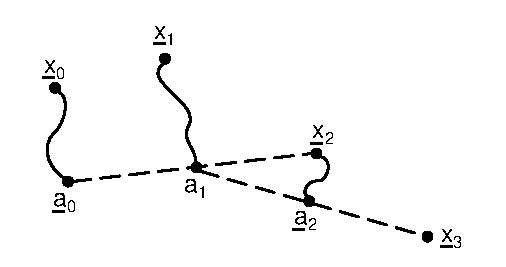
\epsfig{file=mi13.eps}}\end{center}
 
\begin{center}
Fig. 13
\end{center}
\end{figure}
 a `long' random step is taken to the
point ${\underline{x}}_1$, and another rough local minimization is performed to reach the
point ${\underline{a}}_1$(see figure above). Then the so-called `precipitous step' is
taken along a line from ${\underline{a}}_0$ to ${\underline{a}}_1$, some distance past
 ${\underline{a}}_1$ to ${\underline{x}}_2$.
Then from ${\underline{x}}_2$ another rough local
minimization is performed, yielding ${\underline{a}}_2$, and another
precipitous step is taken from ${\underline{a}}_1$ past ${\underline{a}}_2$ to ${\underline{x}}_3$ 
and the search continues in this way.
 
 
      The choice of the `precipitous step' length is important in determining whether the method
will `roll over small ridges, but skirt a high mountain', as its authors say it should. But no
precise way is given, except that `the choice of the length of the precipitous step is carried
out experimentally (by trials) and it constitutes an important
charactistic of the function'.
 
     Moreover, there is no stopping rule, since the method is essentially
searching rather than converging.  In practice one usually stops after
a given length of computer time, but one would also stop if the program
went around in circles repeating itself (which is very possible but not
so easy to detect) or if a predetermined `acceptably small' function
value was attained.  This problem of stopping seems to be common to all
non-local minimization methods.
 
\section{The Goldstein-Price method}
 
     Goldstein and Price \cite{Gold1} have proposed an elegant yet simple method
for seeking other local minima after one local minimum has been found
It is based on a consideration of the analytic (Taylor series) properties
of the function.  Let us assume that the function can be represented as
a Taylor series about a local minimum ${\underline{x}}_1$, where the first derivatives
vanish:
 
$$F({\underline{x}})~=~F({\underline{x}})_1~+~{1\over
2}~({\underline{x}}~-~{\underline{x}}_1)
^T\UTG({\underline{x}}-{\underline{x}}_1)~+~h.t.~.$$
 
Now the higher terms (h.t.), involving third and higher derivatives, are
important since these are the terms that will give rise to other local
minima.  In fact, we seek a way of transforming the function so that only
the higher terms remain.  Such a transformed function is $F_1$ such that:
$$F_1({\underline{x}}_1,{\underline{x}})~=~{2(F({\underline{x}})~-~F({\underline{x}}_1))\over
({\underline{x}}-{\underline{x}}_1)^T\UTG({\underline{x}}-{\underline{x}}_1)}~=~1~+~h.t.~.$$
 By means of this
transformation, we have `removed' the minimum at ${\underline{x}}_1$, and 
the way is cleared to search for other
minima generated by the higher terms of the expansion about ${\underline{x}}_1$.
  The method therefore consists of
seeking a local minimum of the function $F_1$  (It is required to know the
second derivative matrix $\UTG$ at the local minimum ${\underline{x}}_1$.)  Since the
quadratic form $({\underline{x}} - {\underline{x}}_1)^T \UTG({\underline{x}} -
{\underline{x}}_1)$
 is always positive for positive-definite $\UTG$, th
efunction $F_1$ will become negative as soon as an improvement on ${\underline{x}}_1$ is
found.  Then starting from this improved point, the original function $F$
can be minimized locally to yield a new, improved local minimum of $F$.
 
     If the minimum value found for $F_1$ is positive, 
then it may correspond to a new local minimum
of $F$, but not an improvement over ${\underline{x}}_1$.
 
In this case the procedure may be continued from this new point, forming
a new function $F_2$, related to $F_1$ just as $F_1$ was related to $F$. As usual,
no stopping rule is given by the theory.
 
     The method seems to work in practice, although experience with it
is limited and no conditions are known under which it is guaranteed to
work.  It is appealing for reasons of its elegance and simplicity, and
could prove to be an important tool in global minimization.
\newpage
\chapter*{Appendix: Some sample Problems for Minimization Routines}
     We assemble here a collection of test problems  found to be
useful in verifying and comparing different minimization routines.
Many of these are standard functions upon which it has become
conventional to try all new methods, quoting the performance in the
publication of the algorithm.
 
 
\section{Rosenbrock's curved valley}
 
                 $$ F(x,y)~=~100(y~-~x^2)^2~+~(1~-~x)^2$$
\noindent 
start point:{\phantom{xxxxxxxxxxxxxxxxxx}}$ F(-1.2,1.0)~=~24.20$
\vskip2mm
\noindent
minimum:{\phantom{xxxxxxxxxxxxxxxxxxx}}$ F(1.0,1.0)~=~0~.$
\vskip2mm
 
     This narrow, parabolic valley is probably the best known of all test
cases.  The floor of the valley follows approximately the parabola
$y = x^2$ + 1/200, indicated by the dashed line in fig. 14.  In the
cross-hatched area above the dashed line, the covariance matrix is not
positive-definite.  On the dashed line it is singular.  Stepping methods
tend to perform at least as well as gradient methods for this function.\\ \noindent
 [Reference:  Comput. J. {\bf 3}, 175 (1960).]
\begin{figure}[t]
\begin{center}\mbox{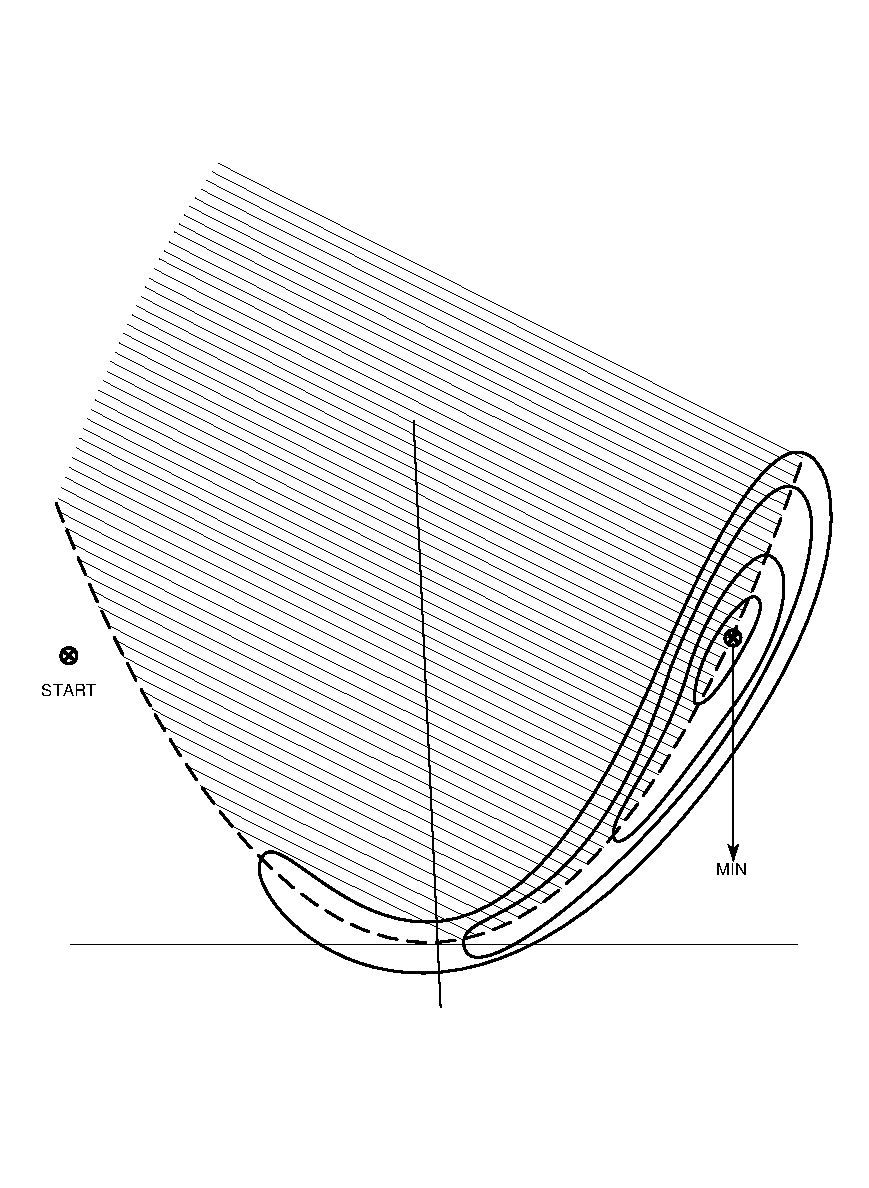
\epsfig{file=mi14.eps,width=10cm}}\\
Fig. 14
\end{center}
\end{figure}
 
 
\section{Wood's function of four parameters}
 
 
\begin{eqnarray}
  F(w,x,y,z)& =& 100(x~-~w^{2})^{2}~+~(w~-~1)^{2}~+~90(z~-~y^{2})^{2}\nonumber\\
              && +~(1~-~y)^{2}~+~10.1[(x~-~1)^{2}~+~(z~-~1)^{2}]~+~19.8(x~-~1)(z~-~1)\nonumber 
\end{eqnarray}
\noindent 
start point:{\phantom{xxxxxxxxxxxxxxxxxx}}$F(-3,-1,-3,-1)~=~19192$
\vskip2mm
\noindent
minimum:{\phantom{xxxxxxxxxxxxxxxxxxx}}$F(1,1,1,1)~=~0~.$
\vskip2mm 
     This is a fourth-degree polynomial which is reasonably well-behaved
near the minimum, but in order to get there one must cross a rather flat,
four-dimensional `plateau' which often causes minimization algorithm to
get `stuck' far from the minimum.  As such it is a particularly good
test of convergence criteria and simulates quite well a feature of many
physical problems in many variables where no good starting
approximation is known.\\ \noindent
[Reference:  Unpublished.  See IBM Technical Report No. 320--2949.]
 
 
\section{Powell's quartic function}
 
 
     $$F(w,x,y,z)~=~(w~+~10x)^2~+~5(y~-~Z)^2~+~(x~-~2y)^4~+~10(w~-~z)^4$$
\noindent 
start point:{\phantom{xxxxxxxxxxxxxxxxxx}}$F(3,-1,0,1)~=~215$
\vskip2mm
\noindent
minimum:{\phantom{xxxxxxxxxxxxxxxxxxx}}$ F(0,0,0,0)~=~0$ .
 \vskip2mm
     This function is difficult because its matrix of second derivatives
becomes singular at the minimum.  Near the minimum the function is given
by $(w~+~10x)^2~+~5(y~-~5)^2$ which does not determine the minimum uniquely.\\ \noindent
 [Reference:  Comput. J. {\bf 5}, 147 (1962).]
 
\section{Fletcher and Powell's helical valley}
 
 
$$F(x,y,z)~=~100\{[z~-~10\Psi(x,y)]^2~+~(\sqrt{x^2~+~y^2}~-~1)^2\}~+~z^2$$
\vskip2mm
\noindent
where 
\begin{tabular}{llll}             
$ 2\pi\Psi(x,y)$ &=& arctan $(y/x)$ &for $x > $0\\
                       &= &$\pi$ + arctan $(y/x)$& for $x < 0$
\end{tabular}
\vskip2mm
\noindent 
start point:{\phantom{xxxxxxxxxxxxxxxxxx}}$F(-1,0,0)~=~2500$
\vskip2mm
\noindent
minimum:{\phantom{xxxxxxxxxxxxxxxxxxx}}$F(1,0,0)~=~0~.$
\vskip2mm 
$F$ is defined only for $-0.25 < \Psi < 0.75$.
 
     This is a curved valley problem, similar to Rosenbrock's, but in
three dimensions.\\ \noindent
[Reference:  Comput. J. {\bf 6}, 163 (1963).]
 
 
\section{Goldstein and Price function with four minima}
 
 \begin{eqnarray}
     F(x,y)&=&(1~+~(x~+~y~+~1)^2 * (19-14x~+~3x^2~-~14y~+~6xy~+~3y^2))\nonumber\\
             &&*~(30~+~(2x~-~3y)^2 * (18-32x~+~12x^2~+~48y~-~36xy~+~27y^2))\nonumber
\end{eqnarray}
\vskip2mm
\noindent
local minima:{\phantom{xxxxxxxxxxxxxxxxxx}}$F$ (1.2, 0.8)~~~~\,= 840\\
{\phantom{xxxxxxxxxxxxxxxxxxxxxxxxxxxxx}}$F$ (1.8,0.2)~~~~~~= 84\\
{\phantom{xxxxxxxxxxxxxxxxxxxxxxxxxxxxx}}$F$ $(-0.6,-0.4)$~= 30\\
global minimum: {\phantom{xxxxxxxxxxxxxx}}$F$ $(0,-1.0)$~~~~~~= 3~.
 
\vskip2mm
 
     This is an eighth-order polynomial in two variables which is well
behaved near each minimum, but has four local minima and is of course
non-positive-definite in many regions.  The saddle point between the two
lowest minima occurs at $F(-0.4,-0.6)$ = 35, making this an interesting
start point.\\ \noindent
 [Reference:  Math. Comp. {\bf 25}, 571 (1971).]
 
 
 \section{Goldstein and Price function with many minima}
 
 
$$F(x,y)~=~\exp \left\{{1\over 2}~(x^2~+~y^2~-~25)^2\right\}~+~\sin^4 (4x~-~3y)~+~{1\over 2}~
(2x~+~y~-~10)^2$$  
 \noindent
 global minimum:{\phantom{xxxxxxxxxxxxxxxxxx}}$F  (3,4)~=~1~.$\vskip2mm \noindent
      This function has `many' local minima.\\ \noindent
[Reference:  Math. Comp. {\bf 25}, 571 (1971).]
 
 
\section{Quadratic function in four parameters}
 
 
 
        $$F(x,y,z,w)~=~{1\over 70}~(21x^2~+~20y^2~+~19z^2~-~14xz~-~20yz)~+~w^2$$
\noindent 
minimum:{\phantom{xxxxxxxxxxxxxxxxxxx}}$ F(0,0,0,0)~=~0$                          
\vskip1cm
\noindent
 covariance~matrix:
 
\hskip10cm
\vskip-2.2cm
\begin{eqnarray*}
\left(\begin{array}{cccc}4&1&2&0\\
1&5&3&0\\
2&3&6&0\\
0&0&0&1
\end{array}
\right)
\end{eqnarray*}
 
     Except for the reasonably strong parameter correlations, this function
poses no special problem to any minimization routine.  But the
author has found it useful in debugging programs based on quadratically
convergent methods, since these programs should minimize the function
exactly in one iteration.  It is also used to check the calculation of
the covariance matrix.
 
     A variation consists of adding $|x|^3~-~1$ whenever $|x| >$ 1, and
similarly with the other variables.  This introduces in a reasonably
smooth way terms which alter the quadratic behaviour far from the
minimum
while leaving it unchanged inside the unit cube, thus providing a test
for those methods which are supposed to converge to the correct
covariance matrix by updating.
 
\section{Chebyquad}
 
 
$$F(\vec{x})~=~\sum^{n}_{i=1}~\left\{\int^1_0~T_i(x^{\prime})~dx^{\prime}~-~{1\over
n}~\sum^{n}_{j=1}~T_i (x_j)\right\}^{2}$$
where $T_i(x)$ are shifted Chebyshev polynomials of degree i;\vskip2mm
\noindent 
start point:{\phantom{xxxxxxxxxxxxxxxxxx}}$x_j~=~j/(n + 1)~.$
\vskip2mm
     This function is designed to have a variable and possibly large
number of parameters, and to resemble functions encountered in actual
practice rather than being contrived to be especially difficult.  Each
term of $F$ represents the squared difference between the true integral
of a polynomial of degree $i$ and the integral estimated by Chebyshev
(equal-weight) quadrature on $n$ points:
 $$\int^{1}_{0}~P(x)~dx~\approx~{1\over n}~\sum^{n}_{j=1}~P(x_j)~.$$
 
The starting values correspond to equally spaced points $x_j$ which is not
too far away from the solution.  Fletcher gives a complete Algol-coded,
procedure for this function in the reference quoted below.\\ \noindent
 [Reference:  Comput. J. {\bf 8}, 33 (1965).]
 
\section{Trigonometric functions of Fletcher and Powell}
$$F(\vec{x})~=~\sum^{n}_{i=1}~\left\{E_i~-~\sum^{n}_{j=1}~(A_{ij}~
\sin~x_j~+~B_{ij}~\cos~x_j)\right\}^{2}~,$$
where
 
 $$E_i~=~\sum^{n}_{j=1}~(A_{ij}~
\sin~x_{0j}~+~B_{ij}~\cos~x_{0j})~.$$
 
$B_{ij} $ and $A_{ij}$ are random matrices composed of integers between -100 and
100;  for $j$ = 1, ..., $n$:  $x_{0j}$ are any random numbers, $-\pi < x_{0j} < \pi;$\vskip2mm
\noindent 
start point:{\phantom{xxxxxxxxxxxxxxxxxx}}$x_j~=~x_{0j}~+~0.1\delta_j, -\pi < \delta j < \pi$
\vskip2mm
\noindent
minimum:{\phantom{xxxxxxxxxxxxxxxxxxx}}$F(\vec{x}~=~\vec{x}_0)~=~0~. $
\vskip2mm 
     This is a set of functions of any number of variables $n$, where the
minimum is always known in advance, but where the problem can be changed
by choosing different (random) values of the constants $A_{ij}, B_{ij}$, and $x_{0j}$. 
The difficulty can be varied by choosing larger starting deviations  $\delta_j$. 
In practice, most methods find the `right' minimum, corresponding to
$\vec{x}~=~\vec{x}_0$, but there are usually many subsidiary minima.\\ \noindent
 [Reference:  Comput. J. {\bf 6} 163 (1963).]
